%% FEUP THESIS STYLE for LaTeX2e
%% how to use feupteses (English version)
%%
%% FEUP, JCL & JCF, 31 July 2012
%%
%% PLEASE send improvements to jlopes at fe.up.pt and to jcf at fe.up.pt
%%

%%========================================
%% Commands: pdflatex tese
%%           bibtex tese
%%           makeindex tese (only if creating an index) 
%%           pdflatex tese
%% Alternative:
%%          latexmk -pdf tese.tex
%%========================================

\documentclass[11pt,a4paper,twoside,openright]{report}

%% For iso-8859-1 (latin1), comment next line and uncomment the second line
\usepackage[utf8]{inputenc}
%\usepackage[latin1]{inputenc}

%% English version

%% MIEIC options
\usepackage[mieic]{feupteses}
%\usepackage[mieic,juri]{feupteses}
%\usepackage[mieic,final]{feupteses}
%\usepackage[mieic,final,onpaper]{feupteses}

%% Additional options for feupteses.sty: 
%% - onpaper: links are not shown (for paper versions)
%% - backrefs: include back references from bibliography to citation place

%% Uncomment the next lines if side by side graphics used
%\usepackage[lofdepth,lotdepth]{subfig}
%\usepackage{graphicx}
%\usepackage{float}

%% Include color package
\usepackage{color}
\definecolor{cloudwhite}{cmyk}{0,0,0,0.025}

\usepackage{pgfplots}
\usepackage{tikz}

\usepackage{float}
\restylefloat{table}
%% Include source-code listings package
\usepackage{listings}

%% MATH packages
\usepackage{amsmath}
\usepackage{nccmath}

\lstset{ %
 language=C,                        % choose the language of the code
 basicstyle=\footnotesize\ttfamily,
 keywordstyle=\bfseries,
 numbers=left,                      % where to put the line-numbers
 numberstyle=\scriptsize\texttt,    % the size of the fonts that are used for the line-numbers
 stepnumber=1,                      % the step between two line-numbers. If it's 1 each line will be numbered
 numbersep=8pt,                     % how far the line-numbers are from the code
 frame=tb,
 float=htb,
 aboveskip=8mm,
 belowskip=4mm,
 backgroundcolor=\color{cloudwhite},
 showspaces=false,                  % show spaces adding particular underscores
 showstringspaces=false,            % underline spaces within strings
 showtabs=false,                    % show tabs within strings adding particular underscores
 tabsize=2,	                    % sets default tabsize to 2 spaces
 captionpos=b,                      % sets the caption-position to bottom
 breaklines=true,                   % sets automatic line breaking
 breakatwhitespace=false,           % sets if automatic breaks should only happen at whitespace
 escapeinside={\%*}{*)},            % if you want to add a comment within your code
 morekeywords={*,var,template,new}  % if you want to add more keywords to the set
}

%% Uncomment to create an index (at the end of the document)
%\makeindex

%% Path to the figures directory
%% TIP: use folder ``figures'' to keep all your figures
\graphicspath{{figures/}}

%%----------------------------------------
%% TIP: if you want to define more macros, use an external file to keep them
%some macro definitions

% format
\newcommand{\class}[1]{{\normalfont\slshape #1\/}}

% entities
\newcommand{\Feup}{Faculdade de Engenharia da Universidade do Porto}

\newcommand{\svg}{\class{SVG}}
\newcommand{\scada}{\class{SCADA}}
\newcommand{\scadadms}{\class{SCADA/DMS}}

%%----------------------------------------

%%========================================
%% Start of document
%%========================================
\begin{document}

%%----------------------------------------
%% Information about the work
%%----------------------------------------
\title{Trustable oracles towards trustable blockchains}
\author{Pedro Duarte da Costa}

%% Uncomment next line for date of submission
%\thesisdate{July 31, 2008}

%%Uncomment next line for copyright text if used
%\copyrightnotice{Name of the Author, 2008}

\supervisor{Supervisor}{Filipe Figueiredo Correia}

%% Uncomment next line if necessary
\supervisor{Second Supervisor}{Hugo Sereno Ferreira}

%% Uncomment committee stuff in the final version if used
%\committeetext{Approved in oral examination by the committee:}
%\committeemember{Chair}{Doctor Name of the President}
%\committeemember{External Examiner}{Doctor Name of the Examiner}
%\committeemember{Supervisor}{Doctor Name of the Supervisor}
%\signature

%% Specify cover logo (in folder ``figures'')
\logo{uporto-feup.pdf}

%% Uncomment next line for additional text  below the author's name (front page)
%\additionalfronttext{Preparação da Dissertação}

%%----------------------------------------
%% Preliminary materials
%%----------------------------------------

% remove unnecssary \include{} commands
\begin{Prolog}
  \chapter*{Abstract}

The Blockchain concept was proposed as a way of processing and recording financial transactions in a peer-to-peer network while avoiding the double-spending problem and without requiring any centralized authority. Later, smart contracts were introduced as immutable applications whose terms are directly written in lines of code that are persisted and run on the Blockchain.

However, currently, smart contracts lack an important feature: internet connectivity. Due to the deterministic nature of Blockchain and the incompatible indeterministic nature of the Web, smart-contracts cannot directly query it.

Oracles solve the connectivity problem, by listening to events produced by smart-contracts, they can insert the needed information on the Blockchain to later be used by the contracts. But oracles do not abide by the same rules and do not support the same guarantees given by Blockchain, so they must either be trusted without hard guarantees about the truthfulness of the data that they provide or we must find ways of guaranteeing their honesty.

In order to find out how blockchain oracles are being designed, a systematic literature review was performed. This review produced fewer oracle solutions than expected, and, therefore, the author also searched for projects created by the industry. Existing oracle solutions rely on two main solutions: authenticity proofs, which are cryptographic proofs that something actually happened, or wisdom-of-the-crowd solutions based on incentives and penalising bad behaviour.
%The former, mostly employed by third-party providers are not fully transparent and always requires some level of trust, and the latter requires a large community and its bad behaviour can go unchecked.

% This text before this is to long on introduction - o texto daqui para cima está demasiado longo, e foca-se muito no background e pouco no SotA. Podes começar por um texto de motivação para o problema, mas podes assumir que as pessoas que lêem o abstract não precisam de encontrar cá a motivação para blockchains e para smart contracts.

% Enumerate architectures in "Secondly, it defines..."

Bearing this in mind, this dissertation contribution is threefold.

Firstly, it analyses and summarises the existing authenticity proofs and mechanisms for guaranteeing oracle trust, allowing a smart-contract developer to be fully informed of the implications of using each proof and their limitations.

Secondly, it defines four possible architectures for oracle design and how each of them addresses different points of trust in the oracle. Starting from the use of a third-party the author identifies and describes two architectures: \textit{Oracle-as-a-Service w/Single Data Feed} and \textit{Oracle-as-a-service w/Multiple Data Feeds}. Then the author describes a self hosted approach with another two architectures: \textit{Single-Party Self Hosted Oracle} and \textit{Multi-Party Self Hosted Oracle}. This way, the author creates a guide that can support those creating blockchain oracles in thinking about the many limitations, trade-offs and possibilities that are inherent to the design of such kinds of system.

Finally, as the author worked on each architecture he found existing oracle solutions that would fit in the first two, regarding third-party providers, and later a new project focusing on the development of the third architecture. Regarding this, the author decided to implement the fourth architecture, both because no existing solution was available and because doing would demonstrate the viability of this new architecture.

In conclusion, this dissertation paves the way for oracle development and research summarising firstly in a broad sense existing solutions and later contributing with a systematic set of architectures and a solution that can be easily adopted by teams interested in deploying their own oracle to achieve higher standards of trust.


\chapter*{Resumo}



%O Resumo fornece ao leitor um sumário do conteúdo da dissertação.
%Deverá ser breve mas conter detalhe suficiente e, uma vez que é a porta
%de entrada para a dissertação, deverá dar ao leitor uma boa impressão
%inicial.

%Este texto inicial da dissertação é escrito no fim e resume numa
%página, sem referências externas, o tema e o contexto do trabalho, a
%motivação e os objectivos, as metodologias e técnicas empregues, os
%principais resultados alcançados e as conclusões.

%Este documento ilustra o formato a usar em dissertações na \Feup.
%São dados exemplos de margens, cabeçalhos, títulos, paginação, estilos
%de índices, etc.
%São ainda dados exemplos de formatação de citações, figuras e tabelas,
%equações, referências cruzadas, lista de referências e índices.
%Este documento não pretende exemplificar conteúdos a usar.
%É usado texto descartável, \emph{Loren Ipsum}, para preencher a
%dissertação por forma a ilustrar os formatos.

%Seguem-se umas notas breves mas muito importantes sobre a versão
%provisória e a versão final do documento.
%A versão provisória, depois de verificada pelo orientador e de
%corrigida em contexto pelo autor, deve ser publicada na página
%pessoal de cada estudante/dissertação, juntamente com os dois
%resumos, em português e em inglês; deve manter a marca da água,
%assim como a numeração de linhas conforme aqui se demonstra.

%A versão definitiva, a produzir somente após a defesa, em versão
%impressa (dois exemplares com capas próprias FEUP) e em versão
%eletrónica (6 CDs com "rodela" própria FEUP), deve ser limpa da marca de
%água e da numeração de linhas e deve conter a identificação, na primeira
%página, dos elementos do júri respetivo.
%Deve ainda, se for o caso, ser corrigida de acordo com as instruções
%recebidas dos elementos júri.
 % the abstract
  \chapter*{Acknowledgements}


\vspace{10mm}
\flushleft{

First of all, I thank my family,

\vspace{5mm}

My father, whose values, ethic and cleverness were always a true example.

My mother, who spends her life helping kids with disabilities become educated man and woman, and whose heart knows no limit.

My brother, whose discipline, brilliance and guidance were always an inspiration.

\vspace{5mm}

These are also the giants in which I proudly stand upon and owe my education to.

\vspace{10mm}

Furthermore, I thank my supervisor Filipe Figueiredo Correia for his guidance, readiness to help and time spent meticulously reviewing this work. I also thank my second supervisor, Hugo Sereno Ferreira, for the productive and challenging discussions we had during critical brainstorming moments.

\vspace{20mm}


Pedro Duarte da Costa}  % the acknowledgments
  \cleardoublepage
\thispagestyle{plain}

\vspace*{8cm}

\begin{flushright}
   \textsl{``If I have seen further it is by standing on ye sholders of Giants.''} \\
\vspace*{1.5cm}
           Isaac Newton
\end{flushright}
       % initial quotation if desired
  \cleardoublepage
  \pdfbookmark[0]{Table of Contents}{contents}
  \tableofcontents
  \cleardoublepage
  \pdfbookmark[0]{List of Figures}{figures}
  \listoffigures
  \cleardoublepage
  \pdfbookmark[0]{List of Tables}{tables}
  \listoftables
  \chapter*{Abbreviations}
\chaptermark{ABBREVIATIONS}

\begin{flushleft}
\begin{tabular}{l p{0.8\linewidth}}
SLR      & Systematic Literature Review\\
HTTPS    & Hyper Text Transfer Protocol Secure\\
TLS      & Transport Layer Security\\
TEE      & Trusted Execution Environment\\
\end{tabular}
\end{flushleft}
  % the list of abbreviations used
\end{Prolog}

%%----------------------------------------
%% Body
%%----------------------------------------
\StartBody

%% TIP: use a separate file for each chapter
\chapter{Introduction} \label{chap:intro}

\section*{}

%O primeiro capítulo da dissertação deve servir para apresentar o enquadramento e a moti\-va\-ção do trabalho e para identificar e definir os problemas que a dissertação aborda. Deve resumir as metodologias utilizadas no trabalho e termina apresentando um breve resumo de cada um dos capítulos posteriores.

%Like the Abstract, the Introduction should be written to engage the interest of the reader. It should also give the reader an idea of  how the dissertation is structured, and in doing so, define the thread of the contents.

Once more, a technological revolution sparked in a not-yet-ready world. Just as the Internet invention brought us closer together and opened an unlimited virtual world of possibilities so does blockchain. The technology is still in its early development days and many different proposals are being worked on to improve its performance and scalability. Akin to the dotcom boom, a plethora of blockchain projects live on more expectations than results but ultimately blockchain could resolve the Internet's failed promise. To understand what is blockchain and why it is necessary we need to comprehend the social background around the time of its release. The Internet promised of a peer-to-peer connected world, however,
 financial incentives and technological challenges led to a centralized and non-privacy advocated virtual world. The increasing general concern regarding the privacy of personal information and the meddling of third parties in everyday online actions allied with the financial crash of 2008 lead to a new technological and social breakthrough.

Satoshi Nakamoto's introduced Bitcoin, in 2009~\citet{Nakamoto2009}, and revolutionized money and currency, setting the first example of a digital asset which has no backing or intrinsic value and more importantly no centralized issuer or controller. In order to require no third party to verify each transaction and prevent double-spending, he introduced a distributed ledger mechanism now known as Blockchain.



\section{Blockchain}

Blockchain is a tool for distributed consensus, in a byzantine fault-tolerant approach, without requiring to trust in centralized parties. In this ledger, transactions are recorded in an ongoing chain, creating an immutable public record that cannot be changed without redoing the proof-of-work. Anyone can become a node and leave and rejoin the network. Having incentives to work on the CPU intensive proof-of-work, extending the chain, and so, for as long as the majority of nodes are trustworthy, the longest and honest chain will thrive. The proof-of-work used on Bitcoin is HashCash, proposed in 1997 by Adam Back, is a cryptographic hash-based proof-of-work algorithm that requires a selectable amount of work to compute, but the proof can be verified efficiently. Nodes can easily verify that a block is valid and that some effort was put in its creation. The proof-of-work difficulty can increase and decrease depending on the network size and capability, creating on average a block every 10 minutes, like a heartbeat.

In simpler terms, transactions are grouped in blocks and for each block there is a mathematical challenge (proof-of-work) which requires time and computational resources to be solved, guaranteeing that some effort is put into solving the challenge and therefore making it extremely hard to quickly manufacture false blocks. Each block has a hash, a signature, of the previous block linking all blocks in a single chain. Nodes always work on the longest chain, so as long as the majority of the nodes are honest and work in building correct blocks, which means they don't have double entries and transactions are legitimate, the biggest chain will grow and remain a trusted and distributed ledger.

Leveraging Blockchain, Bitcoin requires no personal information to exchange value, anyone can join the network and no central authority is needed. This opens an unlimited world of new scenarios for the use of blockchain.



\section{Smart Contracts}

In 2015, Ethereum~\citet{GavinWood2014} was launched as an alternative protocol for building decentralized applications called smart contracts. Introduced as applications that run on the blockchain, smart contracts are self-verifying, self-executing and immutable contracts whose terms are directly written in lines of code which persist on the blockchain, promising to replace real-world contracts. Contracts are the building blocks of our identity, economy and society. They enforce agreements between multiple parties and ensure trust in the compliance of the rules of the agreement but traditional contracts lack automation and decentralization. Smart Contracts provide the ability to execute tamper-proof digital agreements, which are considered highly secure and highly reliable.

Smart contracts have a wide range of use cases. For example, they can be used in Supply Chains and Logistics. Smart contracts allow tracking product movement from the factory to the store shelves. Each intermediary signs a step of the contract which then the final consumer can analyse and have the guarantee of the origin of the product.

\section{The Smart Contract Connectivity Problem}

\begin{figure}[H]
  \begin{center}
    \leavevmode
    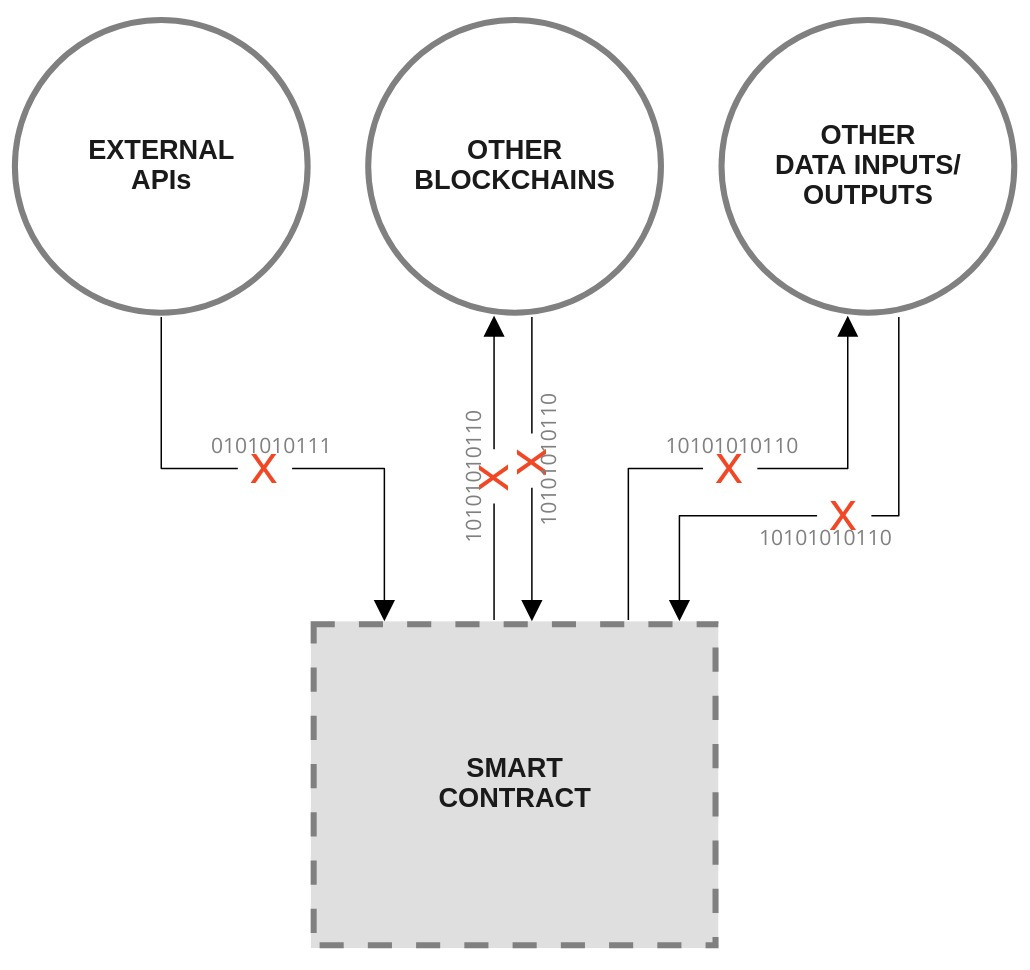
\includegraphics[width=0.7\textwidth]{figures/sc_connectivity.jpg}
    \caption{Smart contract connectivity problem.}
    \label{fig:/figures/sc_connectivity.jpg}
  \end{center}
\end{figure}

The Ethereum blockchain is designed to be entirely deterministic~\citet{GavinWood2014}, meaning that if someone downloads the whole network history and replays it they should always end up with the same state. Bearing this in mind, smart contracts cannot directly query URLs for certain information since everyone must be able to independently validate the outcome of running a given contract making it impossible to guarantee that everyone would retrieve the same information since the internet is non-deterministic and changes over time. Determinism is necessary so that nodes can come to a consensus. In order for smart contracts to gain traction, they need access information of the real world, outside of the blockchain. For example, the current price of the US dollar. However smart contracts cannot directly query the internet for information due to the non-deterministic nature of the internet. Meaning that the information retrieved at some point in time cannot be entrusted to be available or equal in another point in the future, which may result in different states when validating smart contracts by querying the internet in different moments. Oracles solve the non-deterministic problem, of querying the internet, by inputting external information on the blockchain through a transaction making sure that the blockchain contains all the information required to verify itself.


\section{Smart Contracts Space and Computation Limits}

Another problem for smart contracts is performing long and costly operations in terms of computation and space. Several platforms are implementing smart contracts, also called DAPPs, Distributed Applications, namely Ethereum and EOS \citet{Block.one2018}, among others.

On the Ethereum platform, smart contracts pay "Gas" to run. "Gas" is a unit that measures the amount of computation effort that certain operations require to execute. "Gas" is basically the fees paid to the network in order to execute an operation. Therefore, the longer the application runs the more "Gas" the smart contract as to pay.

EOS, on the opposite of Ethereum, works on an ownership model whereby users own and are entitled to the use of resources in proportion to their stake. Basically, instead of paying transaction fees, the owner who holds N tokens is entitled to N*k transactions. While Ethereum rents out computational power on the network, EOS gives ownership of the resources in accordance with the amount of EOS held. The mentioned resources are RAM, corresponding to the used state on the network, CPU measuring the average consumption of computing resources and NET which measures used bandwidth. With increasing prices of EOS tokens, staking these resources becomes very costly.

All in all, either for users of smart contracts or the teams deploying them, keeping smart contracts efficient and performing a non-costly operation is the key. Nonetheless, sometimes applications require costly operations and outsourcing them to an oracle outside of the blockchain is the answer.



\section{Oracles as a Solution}
The solution to the smart contract connectivity problem and to outsourcing computation from the blockchain is the use of a secure blockchain middle-ware, mentioned before as, an oracle. Oracles can query data from APIs, data feeds, other blockchains or perform their own calculations and input that data on the smart contract. This way the blockchain has all the necessary information to verify the result of running a smart contract, and will always produce the same result, independently of the point in time in which that verification runs.


\begin{figure}[H]
  \begin{center}
    \leavevmode
    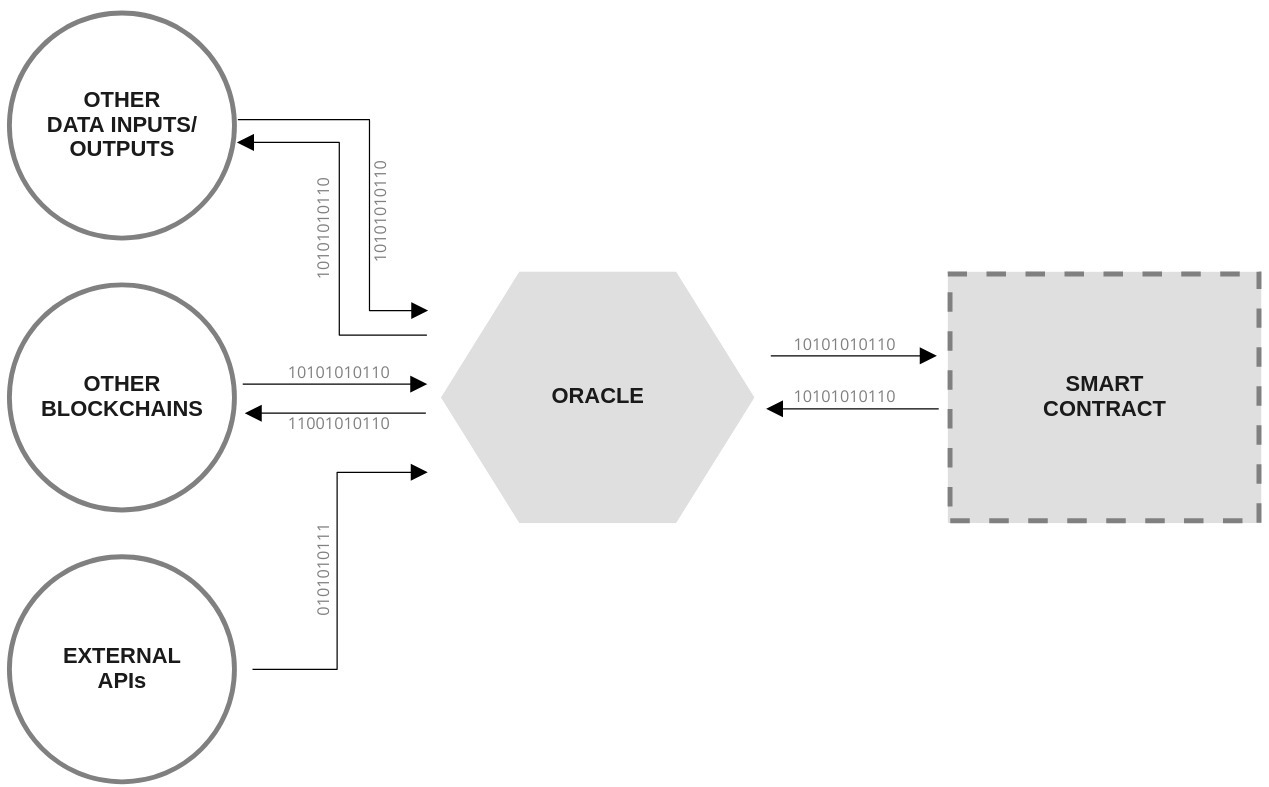
\includegraphics[width=\textwidth]{figures/oracle.jpg}
    \caption{Oracle integration.}
    \label{fig:/figures/oracle.jpg}
  \end{center}
\end{figure}

\section{Authenticity Proofs}
Authenticity proofs, are cryptographic proofs commonly used by oracles in order to prove their honest behaviour. By generating some cryptographic document that can later be used to prove that the oracle actually saw the information that it relayed or computed. In Chapter \ref{chap:chap3} I take a closer look to the existing proofs.



\section{Motivation and Objectives} \label{sec:goals}
The research hereby exposed was proposed by Takai, a blockchain start-up born in Porto, Portugal with the purpose to be the first blockchain open innovation platform. Sponsored by Bright Pixel, an innovation hub and venture investment house, which supports promising startups in their early years. Taikai is building a platform that connects talent and entrepreneurs with the challenges of the corporate players, through the power of the sharing economy and blockchain trust.

The growing interest in blockchain technology and especially in the potential of Smart Contracts together with the lack of research on trustable oracles creates a gap in the general adoption of blockchain by business and governments.

The proposed objectives for this work are as follows:
\begin{itemize}
  \item Defining the requirements for oracle trust;
  \item Understanding blockchain oracles behaviour;
  \item In-depth analysis of existing Authenticity Proofs;
  \item Define several oracle architectures in terms of trust;
  \item Oracle implementation and analysis.
\end{itemize}

\section{Document Structure} \label{sec:struct}

Additionally to the Introduction, this document contains seven more chapters.

In Chapter \ref{chap:sota}, the author analyse the state-of-the-art in terms of blockchain oracles. Initially by performing a systematic literature review, to capture existing academic work on the field and later I expose some more work detailed by companies and individuals in their projects' whitepapers.

In Chapter \ref{chap:chap3}, the author deep-dive on existing authenticity proofs, detailing how they work, what they can achieve and their limitations.

Chapter \ref{chap:chap4} exposes the problem statement underlying this dissertation and exposes a set of forces that are meant to be achieved.

Chapter \ref{chap:chap5} looks at different oracle architectures and their different approaches for achieving trust, assigning a context to be solved by each one and the resulting context of its application.

Chapter \ref{chap:chap6} describes the implementation of the last architecture, creating a simple and effective boilerplate that can be leveraged for a wide range of oracle usage scenarios.

In Chapter \ref{chap:chap7} the author validates each architecture against the forces described in the problem statement, as well as the implementation in its ability to achieve its goal.

Finally in Chapter \ref{chap:concl}, the other concludes on its contributions, details possible future work and describes some of the challenges the author faced during the dissertation. 
\chapter{State of the Art} \label{chap:sota}

\section*{}
%Neste capítulo é descrito o estado da arte e são apresentados trabalhos relacionados para mostrar o que existe no mesmo domínio e quais os problemas em aberto. Deve deixar claro que existe uma oportunidade de desenvolvimento que cobre alguma falha concreta .

%O capítulo deve também efetuar uma revisão tecnológica às principais ferramentas utilizáveis no âmbito do projeto, justificando futuras escolhas.


The topic of blockchain oracles is still unexplored territory mostly investigated by start-up companies and individuals thriving to solve a new problem. Therefore, research related to oracles may not yet be documented on peer-reviewed papers but, nonetheless, is invaluable in an early phase of the technology. Consequently, the state of the art cannot be complete without reviewing the work developed by the academia and also by start-ups, enterprises, governments and individuals. 

\section{Research}
 
To get an overview of academic research a systematic literature review was performed. It's main components and finding are described in this section. 
A literature review allows scholars not to step on each other's shoes but to climb on each other's shoulders \cite{Kitchenham2007GuidelinesEngineering}, meaning, not duplicating existing research and find the gaps and strive to discover something new. To conduct a non-biased, methodical and reproducible review, to the extent that a human can, it is necessary to clarify and identify at the beginning of the research its methodology, what are the data sources and what is the selection criteria.   

\subsection{Research Questions}
First of all and to guide the focus of the research, the following research question was defined:
\begin{itemize}
\item RQ1: What kind of blockchain oracles have been proposed?
\item RQ2: What are the research trends on blockchain oracles?
\end{itemize}


\subsection{Search Strategy and Data-sources}
Figure \ref{fig:/figures/SLR_stages}, presents the predefined review strategy used in order to achieve such a goal and maintain unbiased, transparent and reproducible research.

\begin{figure*}[t]
  \begin{center}
    \leavevmode
    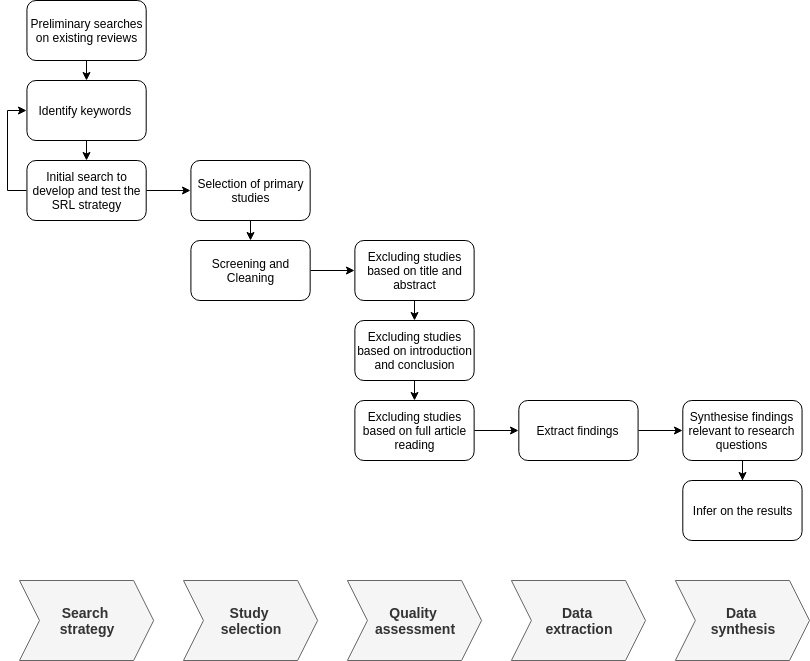
\includegraphics[width=\textwidth]{SLR_stages.png}
    \caption{Review strategy.}
    \label{fig:/figures/SLR_stages}
  \end{center}
\end{figure*}

The following four electronic databases were used to query for such information:

\begin{itemize}
\item ACM Digital Library
\item IEEE Xplore
\item Scopus
\item Google Scholar
\end{itemize}


The defined search query for the search of the relevant papers was the following:

(("blockchain" OR "block chain" OR "block-chain") 
AND 
("oracles" OR "oracle" OR "middle-ware" OR "middleware" OR "middle ware" OR "datafeed" OR "data feed" OR "data-feed"))

This search query was used to comprise all the possible ways of referring to blockchain and oracles. Some scholars have investigated the oracle issue by simply calling them a middleware or data-feed since oracles can either be used as an intermediary that relays data or as the source of the data.

The search was performed on the 5th of February 2019 and revealed the results presented in Table \ref{search-results-table}.

\begin{table}[H]
\centering
\begin{tabular}{llr}
\hline
\textbf{Database} & \textbf{Filters} & \textbf{Results} \\ \hline
ACM Digital Library & Title, abstract and keywords & 34 \\
IEEE Xplore & Title, abstract and index terms & 24 \\
Scopus & Title, abstract and keywords & 57 \\
Google Scholar & Title & 8 \\ \hline
\textbf{Total} & \textbf{} & \textbf{123} \\ \hline
\end{tabular}
\caption{Number of results and applied filters per database}
\label{search-results-table}
\end{table}

Since the concept of smart contracts on the blockchain was only introduced in 2015, with the introduction of the Ethereum blockchain, only results after 2015 were considered, also, all duplicated papers were removed. Analysing the initial search results per year, in Figure \ref{search-results-per-year}, we can infer the growing popularity of oracle-related academic research. The year 2019 only comprises work done in the month of January since the search was performed at the beginning of February. 

\begin{figure}[H]
\centering
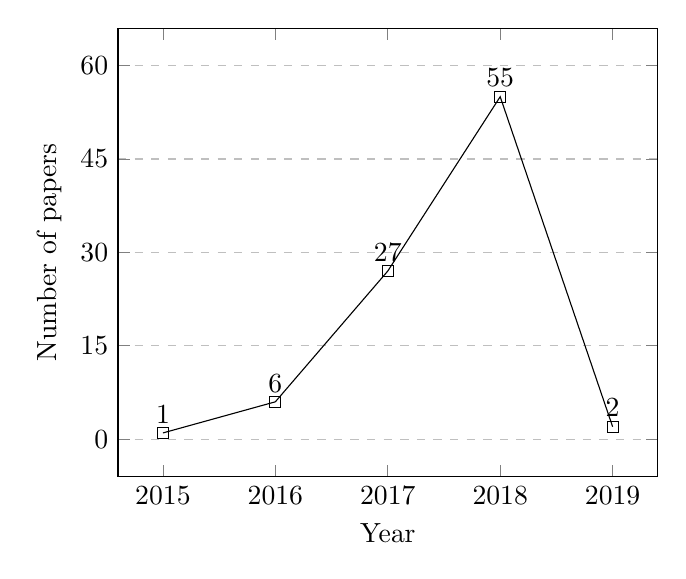
\begin{tikzpicture}
\begin{axis}[
    xlabel={Year},
    ylabel={Number of papers},
    xtick=data, 
    x tick label style={
		/pgf/number format/1000 sep=},
    xmin=2015, xmax=2019,
    ymin=0, ymax=60,
    ytick={0,15,30,45,60,75},
    ymajorgrids=true,
    grid style=dashed,
    enlargelimits=0.10,
]
 
\addplot[
      mark=square, nodes near coords
    ]
    coordinates {
      (2015,1)(2016,6)(2017,27)(2018,55)(2019,2)
    };

\end{axis}
\end{tikzpicture}
\caption{Resulting papers from search distributed per year}
\label{search-results-per-year}
\end{figure}


\subsection{Study Selection and Quality Assessment}

The study selection process initially started with a pool of 123 papers from the previously stated online databases. As described on Figure \ref{fig:/figures/SLR_stages}, the selection compromised four stages:
\begin{itemize}
\item Stage 1: Screening and cleaning duplicated articles or articles that were not in English.
\item Stage 2: Exclusion by carefully reading the title but most importantly the abstract. After this stage, only 13 of the 91 non-duplicated papers were either describing specific trustable oracle implementations or mentioning the use of oracles.
\item Stage 3: Analysing the introduction and conclusions in order to remove papers which do not describe an implementation of a trustable oracle or a protocol to overcome the trust in oracles.
\item Stage 4: Full article reading to assess if the final bucket of articles answers the research questions.
\end{itemize} 

The process of exclusion is depicted in Figure \ref{fig:/figures/paper-screening} and all the information regarding the papers and in which phase they were excluded is transparently presented in Appendix \ref{ap1:slr}.

\begin{figure*}[t]
  \begin{center}
    \leavevmode
    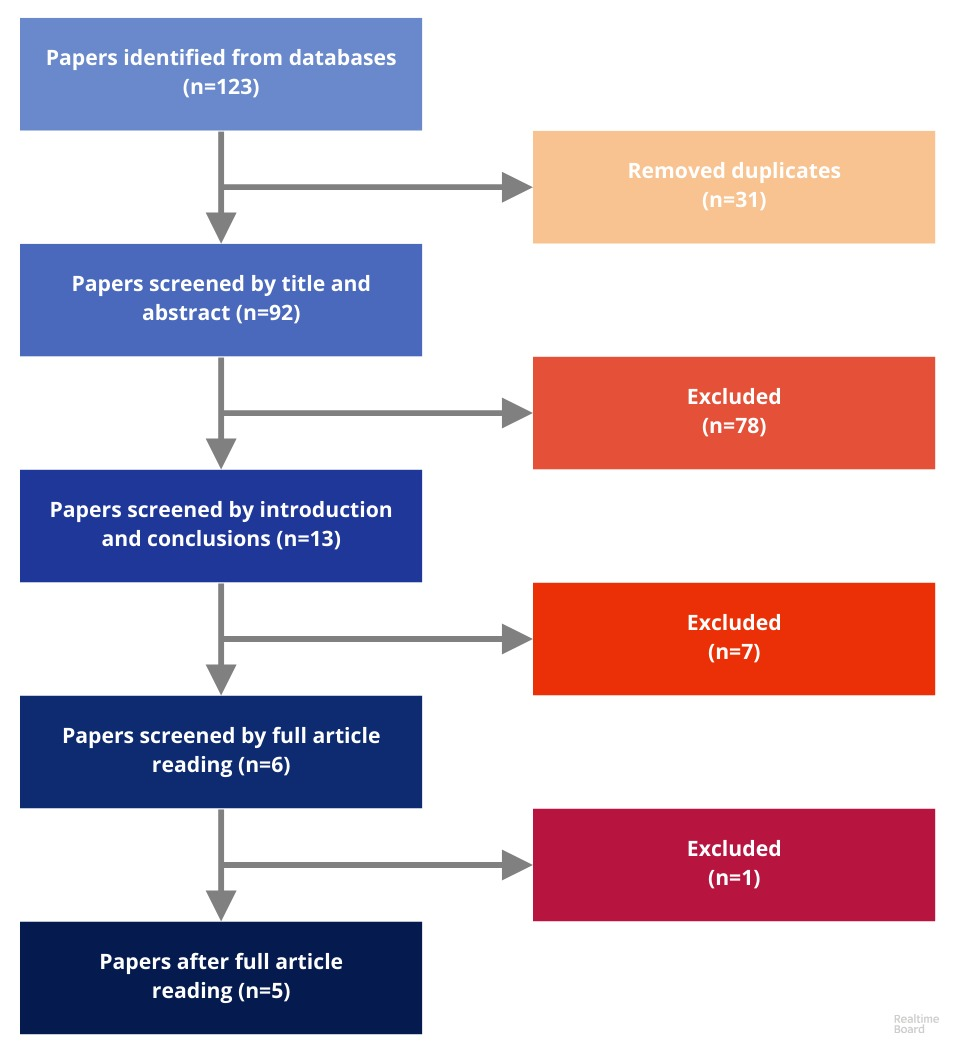
\includegraphics[width=0.7\textwidth]{figures/paper-screening.jpg}
    \caption{Screening stages.}
    \label{fig:/figures/paper-screening}
  \end{center}
\end{figure*}

\subsection{Data extraction and Data Synthesis}

The following process resulted in three articles and two theses that approach varying problems in implementing and guaranteeing trust in oracles.

Town Crier \cite{Zhang2016TownCrier}, leverages trusted hardware, specifically Intel SGX, to scrape HTTPS-enabled websites and serve source-authenticated data to relaying smart contracts. TC architecture involves a TC contract on the blockchain that receives datagram requests from a User Contract on the blockchain and communicates those request to a TC server which then retrieves an answer from a data source through an HTTPS connection.

Astraea \cite{Adler2018Astraea:Oracleb} proposes a decentralized oracle network with submitters, voters and certifiers, in which voters play a low-risk game and certifies a high-risk game with associated resources. Using game theory incentive structure as a means to keep the players honest.

Gilroy Gordon \cite{Gordon2017ProvenanceSensorsb} proposes a protocol for oracle sensor data authenticity and integrity to an IoT devices network with low computational resources. Using sets of public and private keys to authenticate that the oracle sensor data actually was originated by that oracle even if the information needs to pass by several oracles before being consumed by the application.

Francisco Monroy \cite{MontotoMonroy2018BitcoinBlockchain} defines a gambling protocol based on incentives and assuming that every entity involved has the objective to maximize their profit. The protocol overcomes the trust in a single Oracle by polling a network of 7 oracles from a large network of available oracles, they will then stake their money on a specific bet and only receive their investment back if the majority of the oracles vote in the same winner. Creating, therefore, incentives for Oracle good behaviour.

J. Eberhardt \cite{Eberhardt2018Off-chainingComputations} does not propose a specific method but analyses existing solutions and define a systematic classification for existing trustable off-chain computation oracles. The authors identify the following off-chain computation oracles approaches:



\begin{itemize}
\item \textit{Verifiable off-chain Computation}, a technique where a prover executes a computation and then publishes the result including a cryptographic proof attesting the computation’s correctness to the blockchain. An on-chain verifier then verifies the proof and persists the result in case of success. Identified existing solutions are zkSNARKs, Bulletproofs and zkSTARKs. zkSNARKs require a setup phase which is more expensive than naive execution. After the setup, however, proof size and verification complexity are extremely small and independent of circuit complexity. This amortization makes zkSNARKs especially efficient for computations executed repeatedly, which is usually the case for off-chain state transitions. While zkSTARKs and Bulletproofs require no setup, proof size and verification complexity grow with circuit complexity, which limits applicability.
\item \textit{Secure Multiparty Computation}, SMPCs, enable a set of nodes to compute functions on secret data in a way that none of the nodes ever has access to the data in its entirety. Identifies Enigma, which proposes a privacy-preserving decentralized computation platform based on sMPCs where a blockchain stores a publicly verifiable audit trail. However, current sMPC protocols add too much overhead for such a network to be practical. Hence, Enigma now relies on Trusted Execution Environments
\item \textit{Enclave-based Computation}, relying on Trusted Execution Environments (TEE) to execute computations off-chain. Identified existing solutions are Enigma and Ekiden which present two different implementations of EOCs. In Enigma, programs can either be executed on-chain or in enclaves that are distributed across a separate off-chain network. An Enigma-specific scripting language allows developers to mark objects as private and hence, enforce off-chain computation. In contrast to Enigma, Ekiden does not allow on-chain computation but instead, the blockchain is solely used as persistent state storage.
\item \textit{Incentive-driven Off-chain Computation}, IOC, relies on incentive mechanisms applied to motivate off-chain computation and guarantee computational correctness. IOCs inherit two critical design issues: (1) Keep verifiers motivated to validate solutions and (2) reduce computational effort for the on-chain judge. The paper identifies TrueBit, as the first IOC implementation, proposing solutions for both challenges. As verifiers would stop validating if solvers only published correct solutions, TrueBit enforces solvers to provide erroneous solutions from time to time and offers a reward to the verifiers for finding them.
\end{itemize}
  


\section{Non-Academia Research}

To search for non-academic research Google, a search engine and Medium, a platform for blog posting used widely by developers and the start-up community, were used as a means to find new projects or solutions for the oracle trust problem. Using these two tools a lot of projects were found trying to solve the oracle trust problem and are solely documented on white-papers or on the companies website documentation page. This kind of literature cannot be found in peer-reviewed databases, but can nonetheless provide invaluable information and is therefore worth being analysed.

The results of this search revealed a wide range of projects and protocols trying to achieve with varying degrees of decentralization or authenticity, a short explanation of each will be detailed here: 

\begin{itemize}
\item Oraclize.it \cite{Oraclize.it2018OraclizeDocumentation}, provides Authenticity Proofs for the data it fetches guaranteeing that the original data-source is genuine and untampered and can even make use of several data sources in order the gather trustable data, but its centralized model does not guarantee an always available service.
\item ChainLink\cite{Ellis2017ChainLinkNetwork}, describes a decentralized network of oracles that can query multiple sources in order to avoid dependency of a sole oracle which can be prone to fail and also to gather knowledge from multiple sources to obtain a more reliable result. ChainLink is also considering implementing, in the future, authenticity proofs and make use of trusted hardware, as of now it requires users to trust in the ChainLink nodes to behave correctly.
\item SchellingCoin protocol incentivizes a decentralized network of oracles
to perform computation by rewarding participants who submit results
that are closest to the median of all submitted results in a commit-reveal
process.
\item TrueBit, introduces a system of solvers and verifier. Solvers are
compensated for performing computation and verifiers are compensated
for detecting errors in solutions submitted by solvers.
\end{itemize}


\section{Summary and Conclusions}

Summing up, this research highlighted two main types of oracles. The first is \textbf{Data-Carrier oracles}, whose main purpose is relaying query results from a trusted data source to a smart contract. The second is \textbf{Computation Oracles}, which not only relay query results but also perform the relevant computation themselves. Computation oracles can be used as building blocks to construct off-chain computation markets. A summary of the results is described in Table \ref{oracle-summary}.

\begin{table}[]
\centering
\begin{tabular}{llll}
\hline
Name                   & Type         & Distributed Network & Achieves trust through               \\ \hline
Town Crier                         & Data carrier & No                  & Trusted hardware signed attestations \\
Astraea                            & Data carrier & Yes                 & Game theory incentives               \\
\cite{Gordon2017ProvenanceSensorsb}       & Computation  & Yes                 & Sets of public and private keys      \\
\cite{MontotoMonroy2018BitcoinBlockchain} & Data carrier & Yes                 & Incentive based                          \\
TrueBit                            & Computation  & Yes                 & Incentive based                      \\
Oraclize.it                        & Data carrier & No                  & TLSNotary                            \\
ChainLink                          & Data carrier & Yes                 & Query multiple sources               \\
SchellingCoin                      & Computation  & Yes                 & Incentive based                      \\ \hline
\end{tabular}
\caption{Summary of oracle projects/research.}
\label{oracle-summary}
\end{table}

Two main conclusions come from both academic and non-academic research. 

First of all, there is a clear lack of academic research on the topic of creating trustable oracles. Town Crier proposes a solution for relaying data securely but requiring specific hardware. Astraea and \cite{MontotoMonroy2018BitcoinBlockchain} uses incentives and game theory as a means for good oracle behaviour but does not provide complete trust in edge cases in which pursing erratic behaviour may be worth it.

\cite{Eberhardt2018Off-chainingComputations} is very promising in the field of Internet of Things for oracle sensor authentication but can only guarantee that data was generated by a specific sensor but the approach cannot be generalised for other oracle scenarios.

Secondly, even though the main research on trustable oracles is being pursued by startups or sole developers all the existing projects seem to be blockchain specific or in very early phases and not yet ready to be generally adopted.

The literature review points out the lack of research done by the academic in trying to solve one of the most important motives for blockchain general adoption. Only second, maybe, to scalability. The oracle trust problem, efficiently solved, opens doors to the contracts of the futures. Start-ups and sole developers are for now the main force in solving this problem which launches the challenge and motivation for the next chapter of this research.
\chapter{Authenticity Proofs}\label{chap:chap3}

\section*{}

In this chapter, the author takes a deep dive into existing authenticity mechanisms, in terms of their applicability and limitations.

In the context of today's Web, we are accustomed to trusting that a certain website or data is originated from the expected source due to the general adoption of the HTTPS protocol. An extension of the HTTP protocol which creates an encrypted and authenticated channel between the client and the web-server providing the requested information. Then it becomes a matter of whether we trust the source or not, but no doubts are raised as for the channel through which we received it.

Unfortunately, in the context of blockchain, the most used, available and trusted protocols do not have a direct way of communicating with HTTPS enabled services and therefore obtain authenticated data. This creates the need for a trusted service to input that information, but trusting in a third-party service requires it to provide irrefutable proof of its honesty.

Oracles, currently resort to two main techniques to prove their honesty. (1) Authenticity proofs, which is a software or hardware generated cryptographic proof during or after an execution that can later be used to prove the integrity and honesty of the execution or of the provided data. (2) Trusted Execution Environments (TEE) which add another layer of security by isolating the application code from the environment in which it ran, and may also provide cryptographic proof of their honest behaviour.

\section{Trusted Execution Environment (TEE)}
A Trusted Execution Environment is a secure computational environment that is strongly isolated from the main operating system. It provides application isolation, integrity and memory confidentiality. Sensitive data is stored, processed and protected from the main operating system or network. This isolation is accomplished through software and hardware-enforced mechanism. TEE runs a small operating system which exposes a minimal interface to the running application and therefore reduces the attack surface. Advanced TEE embeds unique identities that allow to verify the device authenticity and can be used to generate proofs of the device honest execution.

Examples of TEEs are Intel Software Guard Extensions (SGX)~\footnote{More information on Intel SGX can be found here: https://software.intel.com/en-us/sgx/sdk} and ARM Trustzone-based Secure Elements~\citet{Bunz2018}, the latter is commonly found on smartphones. Another example is Trusty~\footnote{More information on Trusty can be found here: https://source.android.com/security/trusty}, a secure Operating System (OS) that provides a TEE for Android. It is isolated from the rest of the system by both hardware and software. Trusty's isolation protects it from malicious apps installed by the user and potential vulnerabilities that may be discovered in Android.

% FXIME: Confirmar se estas referencias em footnote deveriam estar em referencia mesmo no final

\section{Authenticity Proofs Mechanisms}

Several authenticity mechanisms have been developed and, as described in the state-of-the-art revision, most oracles as a service providers use authenticity proofs to prove their honest behaviour. However, these proofs are not infallible and the details or their implementation are not always transparent or do not provide the disclosed level of trust. I will deep dive on the most common proofs and discuss their implementation and applicability.

\subsection{TLSNotary}\label{proof:TLSNotary}

TLSNotary is a mechanism for independently audited HTTPS (Hyper Text Transfer Protocol Secure) sessions. Allowing clients to provide evidence to a third party auditor that certain web traffic occurred between himself and the server. This mechanism takes leverage of the TLS (Transport Layer Security)~\footnote{Information on the TLS protocol can be found here: https://www.ietf.org/rfc/rfc2246.txt} handshake protocol to create an irrefutable proof, as long as the auditor trusts the server's public key, by splitting the TLS master secret~\footnote{The master secret is used, when generating keys and MAC secrets, as an entropy source, and the random values provide unencrypted salt material and IVs for exportable ciphers.} between three parties: the server, the auditee and the auditor.

The algorithm allows an auditor to verify some part of a session by withholding a small part of the secret data used to set up the HTTPS connection while allowing the client to conduct an HTTPS session normally. The auditor never fully possesses, at any time, any of the session keys and therefore cannot decrypt any sensitive information and can only verify that certain traffic did occur.

\subsubsection{How it works}
TLSNotary modifies the TLS handshake protocol on the client side by levering some properties of TLS 1.0 and 1.1. More specifically the pseudorandom function (PRF) used in the TLS 1.0 RFC 2246.

\begin{ceqn}
    \begin{align}
        PRF(secret,label,seed) = P_MD5(S1,label+seed) \otimes P_SHA-1(S2,label+seed)
    \end{align}
\end{ceqn}

This function compromises two secrets, S1 and S2. The auditor and auditee will independently generate random bytes of data, S1 and S2, respectively.

The auditee applies P\_MD5 to S1, generating 48 bytes:

\begin{ceqn}
    \begin{align}
        H_{1} = H_{1,1} \parallel H_{1,2}
    \end{align}
\end{ceqn}

The auditor applies P\_SHA-1 to S2, generating 48 bytes:

\begin{ceqn}
    \begin{align}
        H_{2} = H_{2,1} \parallel H_{2,2}
    \end{align}
\end{ceqn}


The auditor and auditee then exchange H21 and H12 allowing each other to construct different halves of the master secret, M2 and M1, respectively.

\begin{ceqn}
    \begin{align}
        M_{2} = H_{1,2} \parallel H_{2,2}
    \end{align}
\end{ceqn}

\begin{ceqn}
    \begin{align}
        M_{1} = H_{2,1} \parallel H_{1,1}
    \end{align}
\end{ceqn}

The auditee and auditor calculate X and Y, respectively.

\begin{ceqn}
    \begin{align}
        X = P\_MD5(M_{1})
    \end{align}
\end{ceqn}

\begin{ceqn}
    \begin{align}
        Y = P\_SHA-1(M_{2})
    \end{align}
\end{ceqn}

The auditor sends sufficient bytes from Y to the auditee so that it can compute the necessary encryption keys and client mac key to send the request to the server.

Then the server response is received, but not decrypted, and the network traffic is logged and a hash of the traffic is computed and set to the auditor as commitment.

Only then, does the auditor send the remaining bytes of Y to the auditee and this allows him to calculate the server mac key and safely execute the regular TLS decryption and authentication steps.

This complex sequence of calculations prevents the auditee from creating a fake version of the post-handshake traffic from the server since he did not have in his possession the server-mac-write-secret to decrypt and authenticate the initially requested data.

\subsubsection{Limitations}
TLSNotary provides some capabilities to attest TLS connections but comes with several limitations. Firstly, TLSNotary supports only TLS 1.0 or 1.1, the properties mentioned before are not present in TLS 1.2 and 1.3 and the former are considered less secure versions of TLS. Secondly, TLSNotary depends on RSA Key exchange, which does not provide forward secrecy. Thirdly, TLSNotary uses MD5 and SHA-1 functions, which are now considered deprecated. Finally and most importantly, TLSNotary requires trusting in a third party in most of its implementations, such as in Oraclize~\cite{Oraclize.it2018}, and being an interactive proof there is no way to verify the TLSNotary proof unless you were performing the role of the auditor during the retrieval. Oraclize, runs an auditor node on Amazon Web Services (AWS), claiming that this implementation is secure as far as AWS is trusted, simply moving the trust to a larger central entity. It also only allows the existence of one auditor in which we must trust, TLSNotary will not be a suitable solution if more than one auditor is required.


\subsubsection{Conclusions}
The TLSNotary proof is promising due to be software based and is, as of this moment, the most spoken of authenticity proof. However, it's applicability is increasingly getting limited due to the deployment of new TLS versions and the assurances provided by the proof current implementations, which simply move the trust to a bigger entity. Therefore, it should not be considered a reliable authentication method for future implementations.

\subsection{Android Proof}

In the oracle context, the Android Proof \footnote{Documented explanation of the proof can be found here: https://provable.xyz/papers/android\_proof-rev2.pdf} results from Oraclize research and development efforts. It takes leverage of SafetyNet software attestation and Android Hardware Attestation to provision a secure and auditable environment to fetch authenticated data.

\subsubsection{SafetyNet Attestation}
SafetyNet~\footnote{Further described on the google developer page: https://developer.android.com/training/safetynet/attestation.html}, developed by Google, is an API service that allows assessing the Android device in which an app is running on. It provides a cryptographically-signed attestation, assessing the integrity of the device, looking at the software and hardware environment for integrity issues. By returning an SHA-256 hash of the application that called the SafetyNet API it allows assessing if the application running on the device has not been tampered with by comparing the application SHA-256 hash with its publicly available and distributed open-source code.

\subsubsection{Android Hardware Attestation}
Since Android Nougat~\footnote{https://www.android.com/versions/nougat-7-0/}, developers are able to generate an hardware attestation object with details regarding the device unique key stored in the Android Hardware KeyStore~\footnote{Further explanation can be found here: https://source.android.com/security/keystore/}. The attestation object is signed by a special attestation key kept on the device and the root certificate used by that key is a known Google certificate. This guarantees that the hardware running the code has not been tampered with.

\subsubsection{How it works}
The application running on the Android device, on its first run, creates a NIST-256p key pair, containing the Hardware Attestation Object to prove the integrity of the key, using the Android Hardware KeyStore.

When a request is sent to the Android device, it starts an HTTPS connection and the entire HTTP response is retrieved. The response's SHA256 hash is signed using the hardware attested key pair created on the application start. A call to SafetyNet API is then issued to attest the SHA-256 hash of the application package running on the device, which should be open-source and public available and distributed, guaranteeing the application integrity and therefore that no change has occurred on the HTTP response before it was signed and its hash used in the SafetyNet request.

SafetyNet then returns an attestation response in the JSON Web Signature format (JWS) that guarantees the integrity of the application running, the integrity of the system in which the application ran and that both the HTTPS request and the signing process using the initially created and attested key has taken place in the application issuing the SafetyNet request.

The SafetyNet JWS response and the HTTP response is sent back for off-chain verification and validation.

\subsubsection{Conclusions}
The Android proof is a far more complex and in-depth authenticity proof in comparison to TLSNotary. It provides strong guarantees of software and hardware integrity as well as of the requested data. Nonetheless, it relies on a centralized authority, Google, to develop a secure Trusted Execution Environment (TEE), used by Android to generate private keys, and to maintain SafetyNet security sophisticated enough to offer good guarantees of the device and application integrity. A bottleneck in this approach can be the required use of a physical Android device, limiting the scalability context of this approach, but nonetheless, as long as Google is trustworthy it is a very secure model.

\subsection{Ledger Proof}

The ledger proof is based on the use of a specific trusted environment, the Ledger Nano S~\footnote{https://shop.ledger.com/products/ledger-nano-s} and Ledger Blue~\footnote{https://shop.ledger.com/products/ledger-blue}, developed by a French company to secure crypto assets safely. This device provides an attestation for its authenticity and code integrity.

\subsubsection{How it works}

This device implements several layers of hardware and software to prove the security of its execution. These devices run specific software, BOLOS~\footnote{Specific information regarding BOLOS can be found here: https://ledger.readthedocs.io/en/0/bolos/index.html} (Blockchain Open Ledger Operating System), which has an SDK that enables developers to build application which can be installed on the hardware. BOLOS exposes a set of kernel-level APIs which allows running secure cryptographic operations as well as attest the device and the code running on it. The later is very useful as it allows to run code in a secure manner and provides an attestation for the code. An application can ask the kernel to produce a signed hash of the application binary code. A special attesting key is used in this process and is safely controlled by the kernel, away from attacks attempts by any application code. With this, the ledger proof leverages both the device attesting and code attesting features to prove that the applications are running on a TEE of a ledger device.

\subsubsection{Conclusions}

Currently, the ledger proof is used by Oraclize to provide true random data to a smart contract. But its use can be extended to other computation operations that may require to run outside of the blockchain as long as there is support in terms of computational and memory capacity by the ledger device. The device also lacks a direct connection to the internet and therefore cannot be used to query data from the internet.


\subsection{TLS-N}

TLS-N \cite{Ritzdorf2017}, is the first privacy preserving TLS extension that is efficient and most importantly provides non-repudiation~\footnote{Non-repudiation refers to a state of affairs in which the authenticity of something cannot be challenged, meaning that there is absolute guarantee that something happened the way that it is stated.}. TLS-N does not require the use of a third-party or any trusted hardware and is an extension to the TLS 1.3 protocol. In comparison to other implementations such as TLSNotary which rely on deprecated versions, is up to date to the current technologies.
It guarantees non-repudiation, not only in a single TLS message exchange but also in a conversation compromising several messages. It allows, with an additional computation overhead, to obfuscate certain parts of the conversation (such as passwords or other sensitive information) while keeping its trust model intact.

In the TLS-N model, there is no need to trust in a single auditor, such as in TLSNotary, since the proofs are non-interactive and can be inspected by anyone, at any point in time, without having to trust in a single auditor honesty.


\subsubsection{How it works}
TLs-N requires the web server (generator) and the client (requester) to have both support for the protocol.

Initially, both generator and requester establish a TLS connection and negotiate the TLS-N parameters in the handshake. The generator stores the state of the conversation which comprises a hash value incorporating all previous records, an ordering vector and the time stamp from the start of the session.

The protocol ends when the requester sends a request for evidence. The evidence is composed of a window of the exchanged ordered messages signed by the generator. The window begins right after the handshake, this prevents Content Omission Attacks, depicted on Figure~\ref{fig:/figures/tlsn-content-omission}.

\begin{figure*}[h]
    \begin{center}
        \leavevmode
        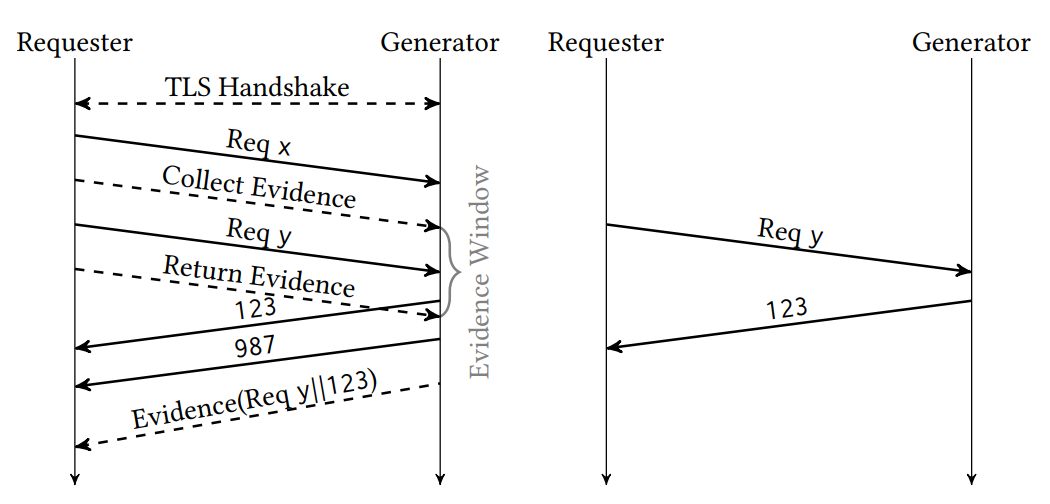
\includegraphics[width=0.9\textwidth]{figures/tlsn-content-omission.PNG}
        \caption{Content Omission Attack - The left figure shows the original and the right figure the signed conversation.}{Image extracted from \citet{Ritzdorf2017a}}
        \label{fig:/figures/tlsn-content-omission}
    \end{center}
\end{figure*}

In this situation the evidence collection only starts after the first request is done, and another request is asked right after (this one, inside the window collection, Req y on the image) and the response for the first request is assumed to be the response to the second one. Only this two messages are stored in the evidence window, since context is missing in the signed conversation, the response 123 appears to belong to request y which is incorrect. Therefore, TLS-N always starts right after the TLS handshake. The correct TLS-N flow is presented on Figure~\ref{fig:/figures/tlsn-normal-flow}.


\begin{figure*}[h]
    \begin{center}
        \leavevmode
        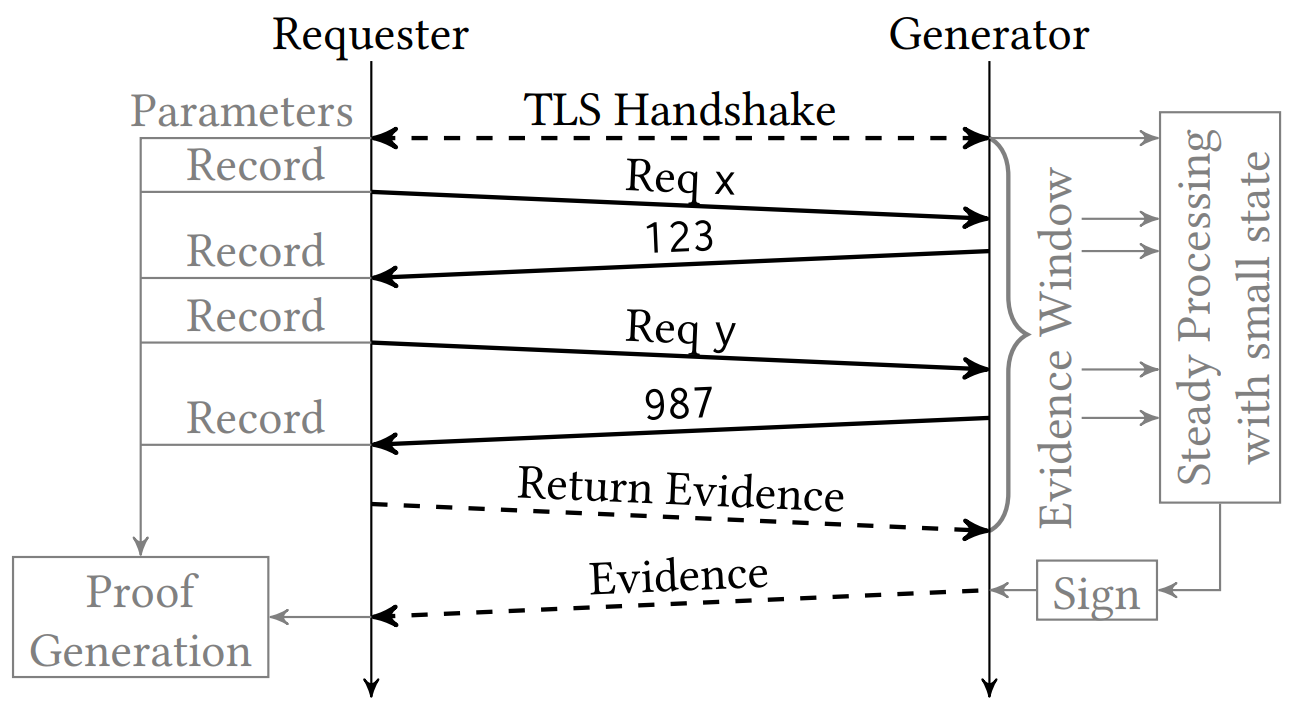
\includegraphics[width=0.7\textwidth]{figures/tlsn-normal-flow.PNG}
        \caption{Simplied Overview of TLS-N.}{Image extracted from \citet{Ritzdorf2017a}}
        \label{fig:/figures/tlsn-normal-flow}
    \end{center}
\end{figure*}

To generate a small proof independently of the number of messages, TLS-N uses merkle trees~\cite{MerkleTrees} to create a chain of messages' hashes and then returns only the last hash, which to be created requires all the previous hashes. This ensures a small storage overhead per TLS session.


\subsubsection{Conclusions}
TLS-N was designed with the oracle trust problem in mind, the generated proof is small enough to be evaluated on-chain on a smart-contract. The only drawback is that the smart contracts cannot verify TLS signatures based on the web-PKI (public-key infrastructure) and therefore the contract must have the generator public key.

TLS-N is, therefore, a promising solution to the oracle trust problem being the only major drawback requiring the data providers to adopt the TLS-N protocol.


\subsection{Town Crier}

Town Crier~\citet{Zhang2016a} (TC) authenticates data-feeds through the use of trusted hardware, more specifically Intel SGX enabled CPUs. By levearing intel SGX, and as long as this system is trusted, there's is no need to trust the environment in which TC is running since it the TEE guarantees the isolation of the TC implementation.

Thanks to its use of SGX and various innovations in its end-to-end design, Town Crier offers several properties that other oracles cannot achieve:

\begin{enumerate}
    \item \textbf{Authenticity guarantee}: There's no need to trust any particular service provider(s) in order to trust Town Crier data. (You need only believe that SGX is properly implemented.)
    \item \textbf{Succinct replies}: Town Crier can prune target website replies in a trustworthy way to provide short responses to queries. It does not need to relay verbose website responses. Such succinctness is important in Ethereum, for instance, where message length determines transaction costs.
    \item \textbf{Confidential queries}: Town Crier can handle secret query data in a trustworthy way. This feature makes TC far more powerful and flexible than conventional oracles.
\end{enumerate}

\subsubsection{How it works}

Intel’s Software Guard Extensions (SGX) is a set of new instructions that confer hardware protections on user-level code. SGX enables process execution in a protected address space known as an enclave. The enclave protects the confidentiality and integrity of the process from certain forms of hardware attack and other software on the same host, including the operating system.

Upon request, the enclave can generate a proof, usually called attestation, signed by and hardware protected key that can be used to prove that a certain software was run in a legit TEE.

The flow of a TC requests starts with a User Contract creating a datagram request to the TC Contract. The TC Contract, is a simple smart-contract on the blockchain that accepts client requests and to whom the TC server listens to for new requests.

The TC Server, listens to events on the TC Contract and queries the requested data-source. The enclave takes care of signing the operation where as the relay is a simple networking interface. The answer is signed and returned to the TC Contract to later relay it to the User Contract.



\subsubsection{Conclusions}
Town Crier, presents an effective solution to tackle trust issues in the oracle operation. It does require the use of proofs as well as its later analysis for good behaviour and specific hardware.

In scenarios, where there is a higher requirements for trust in the oracle behaviour and cost/performance is not a problem, TC is a viable and more secure solution than software-based proofs.


\section{Summary}

Table \ref{tab:summary-proofs} summarizes the previous analysed proofs regarding the necessities of specific hardware, the possibility of their usage to not be deprecated in the next following years, if whether they can query the web and are already be used in production.

\begin{table}[]
    \centering
    \resizebox{0.95\textwidth}{!}{%
        \begin{tabular}{@{}lcccc@{}}
            \toprule
            Proof         & \multicolumn{1}{l}{Requires specific hardware} & \multicolumn{1}{l}{Can query the Web} & \multicolumn{1}{l}{Future-proof} & \multicolumn{1}{l}{Currently in production} \\ \midrule
            TLSNotary     &                                                & X                                     &                                  & X                                           \\
            Android Proof & X                                              & X                                     & X                                & X                                           \\
            Ledger Proof  & X                                              &                                       & X                                & X                                           \\
            TLS-N         &                                                & X                                     & X                                &                                             \\
            Town Crier    & X                                              & X                                     & X                                & X                                           \\ \bottomrule
        \end{tabular}
    }
    \caption{Summary of authenticity proofs}
    \label{tab:summary-proofs}
\end{table}



%FIXME: Falta aqui um texto a comparar as várias opções, se possível ilustrado por uma tabela de síntese em que se mostre rapidamente em que pontos são semelhantes e diferentes
\chapter{Problem Statement}\label{chap:chap4}

\section*{}

%% FIXME: Problem chapter
%O capítulo sobre o problema que devia aparecer neste ponto, precisa de conter:
% - descrição geral do problema (possivelmente repetindo um pouco, mas não inteiramente, do que foi dito no capítulo da introdução) e âmbito que pretendemos atacar
% - a hipótese central subjacente ao trabalho
% - as sub-hipóteses ou research questions mais concretas
% - qual a estratégia de investigação que será usada

Smart contracts power a decentralized world of automation and trust-less commitments. Companies, groups and individuals are able to automate tasks and contracts but as far as the ecosystem is, smart contracts are still very much limited to the information available in the blockchain. Therefore, connecting with the outside world requires a trusted authority to input in the blockchain the required information upon request from the smart contract. This trusted authority is generally called an oracle.

As explained before, the deterministic nature of blockchain does not allow smart contracts to directly query a data-feed for information. In this context, oracles help connecting smart contracts to the world outside of the blockchain. The problem here is to trust in the oracle service to not behave maliciously and undermine the trust provided by the blockchain consensus mechanisms. Blockchain technology can be trusted to behave correctly even in byzantine environments, but the oracle service does not abide by the same mechanisms and therefore some mechanisms must be put in action to ensure the oracle's response credibility.


%% acredito que ao fazer x tenho y beneficios

\section{Forces}
\begin{itemize}
    \item \textbf{Smart contract empowerment} - Providing smart contracts with trustable information from outside of the blockchain is decisive to gain general adoption and practicality.
    \item \textbf{Blockchain interoperability} - The ability to get information from other blockchains if possible using an oracle that queries one blockchain and inputs the information on another.
    \item \textbf{Keeping trust standards} - As blockchain technology creates a trust-less environment, oracles should as well keep up with the level of trust in their functioning.
\end{itemize}

\section{Proposal}

With this thesis, I intend to lay the foundations for the development and architecture of trustable oracle systems that will power several use cases and smart contracts. By describing in a trust-guided manner multiple patterns and examples where they are being applied or possible use cases not yet documented. This guided model should help future cases to have a systematic approach to which architecture will fit the best to each case.

Furthermore, I will present a possible implementation of a self-hosted oracle. As the following architectures and previous analysis of autenticity proofs point out, the best way to have trust in an oracle is to deploy one instead of relying on an oracle service. This approach reduces operations costs and empowers the contract with a purpose built oracle.

\chapter{Trustable Oracles }\label{chap:chap5}

\section*{}

At this point, a definition, of what trust in an oracle is, seems appropriate. Trust has a lot of meanings, depending on the needs of all the parties involved. I will model several levels of trust and the requirements and fallacies of each model as well as its application and drawbacks.

Starting from an absolute trust scenario, in this model, the end user, being the smart contract which receives information provided by the oracle, has complete assurances from both the veracity of the data provided by the data source, as well as, undeniable proof that the oracle did not tamper with the relayed information. This scenario points out two main points of failure, either maliciously or unintentionally.

The first component which can be faulty or compromised is the data source. Assuring that the information provided is correct does not have a straightforward answer. What correct means is open to interpretation. For example, if the data source is an IoT sensor, which is prone to failures, being correct is relative. The sensor needs to be perfectly calibrated and accurate. In this case, using several sensors and averaging its values or removing outliers would solve its correctness. Another example could be an API that returns the current value of the EUR in USD. In this scenario, a party that would benefit from a higher conversion than the real one could coerce or attack the data-source into providing a favourable value. The answer here can also be using several data sources. Another solution would be to use a highly trusted entity such as the European Central Bank (ECB) which can be a lot harder to coerce or attack and having a signature from the ECB that backs the provided data. Choosing what type of data-source to use has a huge impact on the trust fullness of the provided data not to mention architecture centralization when using a source such as the ECB. All in all, the end user will have to understand the requirements and level of trust necessary.

The second, and most relevant for analysis, is the oracle service used. Oracles are a necessary part of the process since the other option would be having the data providers adapting to the blockchain which does not seem to be a realistic option at the moment. Therefore we must trust an oracle or a group of oracles. Two main options are available, either trusting a third-party oracle or self-deploying an oracle. In the first scenario, three variables take part in the level of trust. Firstly he third-party oracle, if paid for, has the monetary incentive to be honest, since a bad record of dishonesty would have the service losing credibility and therefore clients. Secondly, by using proofs the oracle can establish its legitimacy, as long as, the proofs can undoubtedly be trusted and verifiable by the smart contract, I will later analyse in depth this issue. Finally, oracle execution transparency by using open-source code and having means for being audited. Additionally, to guaranteeing single oracle integrity, it may be in the interest of the user to use several oracles either to provide service availability or to increase trust by combining the result from different oracle services.


\section{Oracle Architectures}

Having analysed what trust means, it is evident that no short definition is appropriate and that it depends on the stakeholder beliefs. Hence, several architectural models for what a trustable system arise. Varying in decentralization and complexity. Each model satisfies different requirements, such as performance, security and decentralization.
In this section, I will describe several possible architectures and point out use cases and compromises for each model.

% FIXME: Explain the structure of the architecures

\section{Oracle as a Service w/ Single Data Feed.}\label{OaaSwSingleDataFeed}

\subsection{Context}
Connecting smart contracts with information provided by data-feeds, which do not, by themselves, input the required information on the blockchain requires the use of a trusted oracle. Developing and maintaining a oracle may be prohibitive in terms of cost (if assembling a team was needed) and desired time to market. Outsourcing such service would be desirable in this context, it may not be in the interest of the company to specialize in the secure development of oracles.

\subsection{Example}
A smart contract developer needs to obtain information from an API source without having the trouble to develop and launch its on oracle whilst having some guarantees of the origin of the information. Mainly, this scenario is focusing on fast-time to market, untampered data and cost is not a problem.


\subsection{Problem}
How can a non-blockchain company keep up with the fast pace of industry while maintaining trust in its services? It is critical to be able to quickly build a smart contract and connect it with the needed information. How can a company do so, without allocating human resources into to the development of yet another service and simply focus on its business logic?

\subsection{Forces}

\begin{itemize}
  \item \textbf{Fast time-to-market} - Quickly deploy a product without the overhead of focusing on oracle functionality and security.
  \item \textbf{Trust} - The oracle should guarantee as much as possible the same level of trust in its functioning as the underlying blockchain technology.
\end{itemize}


\subsection{Solution}
Oracle as a service, come as a quick and efficient solution for fast moving companies and individuals. Providing easy integration between a smart contract and a data-feed by means of specific function calls and/or libraries. Theses services are per-request fee-based and can be cheaper comparing to assembling a team dedicated to the development and maintenance of an oracle. The fee-based system increases the trust in the service as being honest is crucial to their business model. Additionally, this services usually provide authenticity proofs which serve as another layer of trust in the service. In the Chapter \ref{chap:chap4} I deep dive on the subject of the proofs.

\begin{figure*}[t]
  \begin{center}
    \leavevmode
    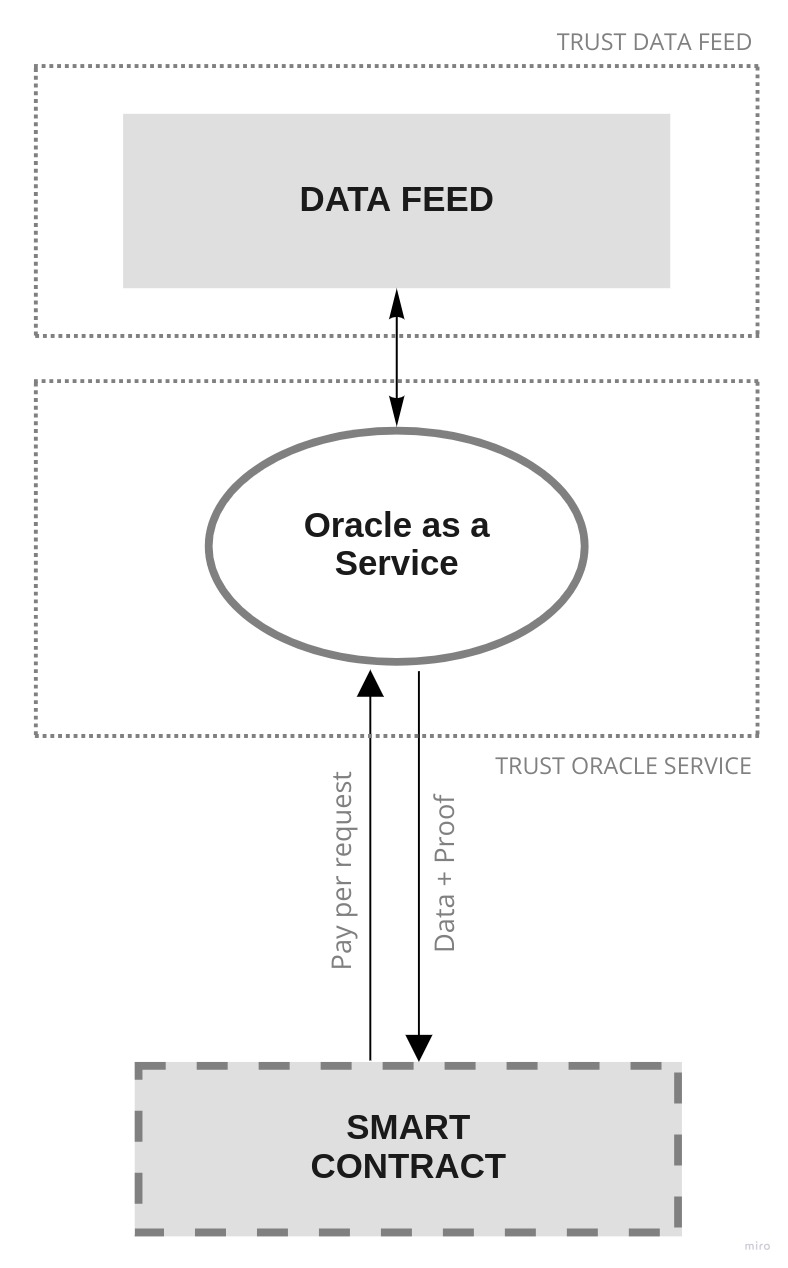
\includegraphics[width=0.5\textwidth]{figures/oraclearch1.jpg}
    \caption{Oracle as a Service w/ Single Data Feed.}
    \label{fig:/figures/OaaSwSingleDataFeed}
  \end{center}
\end{figure*}

\subsection{Example Resolved}


\subsection{Resulting Context}
%% FIXME: o resulting context muitas vezes foca-se nos "quality attributes" (e.g., trust, reliability, resilience, cost) que são característica da solução. ao ler esta secção fico a achar que estas características estão de facto aqui descritas, mas às vezes é preciso ler nas entrelinhas quais são. uma forma de as tornar mais visíveis é estruturar este texto como bullet points (um ponto por quality attribute); outra forma é de formatar a bold as palavras que identificam esses quality attributes

This solution results in an architecture that compromises two points of trust. The first being the data-feed itself. No guarantees are given that the data provided is reliable and the smart contract owner must, therefore, to the best of his knowledge, select a data-feed in which, by the operator size or record of good behaviour, he can trust.

The second point of failure is the oracle service itself. Although smart contracts, in the resulting context, have access to the information from the outside, that is only possible due to the use of a third party to honestly relay the data. In this architecture, if the oracle simply relays the data, then no trust model can be achieved as the oracle good behaviour is not tested against. As this would not be a feasible architecture the existing services provide authenticity proofs to guarantee, to a certain level, their honest behaviour. The problem here is on how are these proofs generated, can they be verified on-chain or only off-chain and who is making, or providing, the verification tools. In Chapter~\ref{chap:chap4} I deep dive on these questions and techniques. Another reason to trust in the service can be the monetary incentive for good behaviour. By paying the oracle for each request, that becomes the oracle service business model, an extensive record of good behaviour is crucial for business prosperity and therefore a good enough incentive for honestly conveying the requested data.
In this context, if the authenticity proofs provide enough assurances for the smart contract creator and he trusts in the selected data-feed to provide the required data, then this model can satisfy its needs in terms of trust, as well as, performance since it only queries one data-feed and uses only one oracle. By not having any consensus mechanism an exchanging the least amount of messages it can both achieve greater performance and a lower cost. But this lower cost and higher performance architecture by itself is prone to failure due to lack of decentralization and does not guarantee service availability which could lead to a failure in the smart contract to obtain the requested information.

\subsection{Known Uses}
%% FIXME: Mention oraclize here


\section{Oracle as a Service w/ Multiple Data Feeds.}\label{OaaSwMultipleDataFeed}

\subsection{Context}
This scenario iterates on the previous one but focuses on data veracity. Sometimes an answer to a contract request cannot be truly accepted unless several sources confirm it. Either because it is unwise to trust in a single identity or because there might not be a single true answer but only an answer that is accepted by a selected majority.

\subsection{Example}

\subsection{Problem}
The previous architecture specified a single point of failure on the data-source layer. A contract with high requirements in terms of availability cannot rely on using a single data-source, as doing so would void the contract when the service providing that data is down or taken down. In terms of trust, certain contracts may also require that several services provide an answer and then have a consensus between all the received answers. This cannot be achieved by querying a single source and therefore the oracle service must be able to query several sources and either define the resulting answer or provide all the responses to the smart contract and let the smart contract resolve to a final answer.

\subsection{Forces}
\begin{itemize}
  \item \textbf{Availability} - Higher fault-tolerance guarantees in the data provider.
  \item \textbf{Trust} - Higher trust on the veracity of the queried data..
\end{itemize}

\subsection{Solution}
The oracle service should have a mechanism to query several data-sources during a specified timeframe. And have a predefined consensus mechanism that would require to have m of n data-sources providing the possible answers and reduce them to a final answer to the smart contract.


\begin{figure*}[t]
  \begin{center}
    \leavevmode
    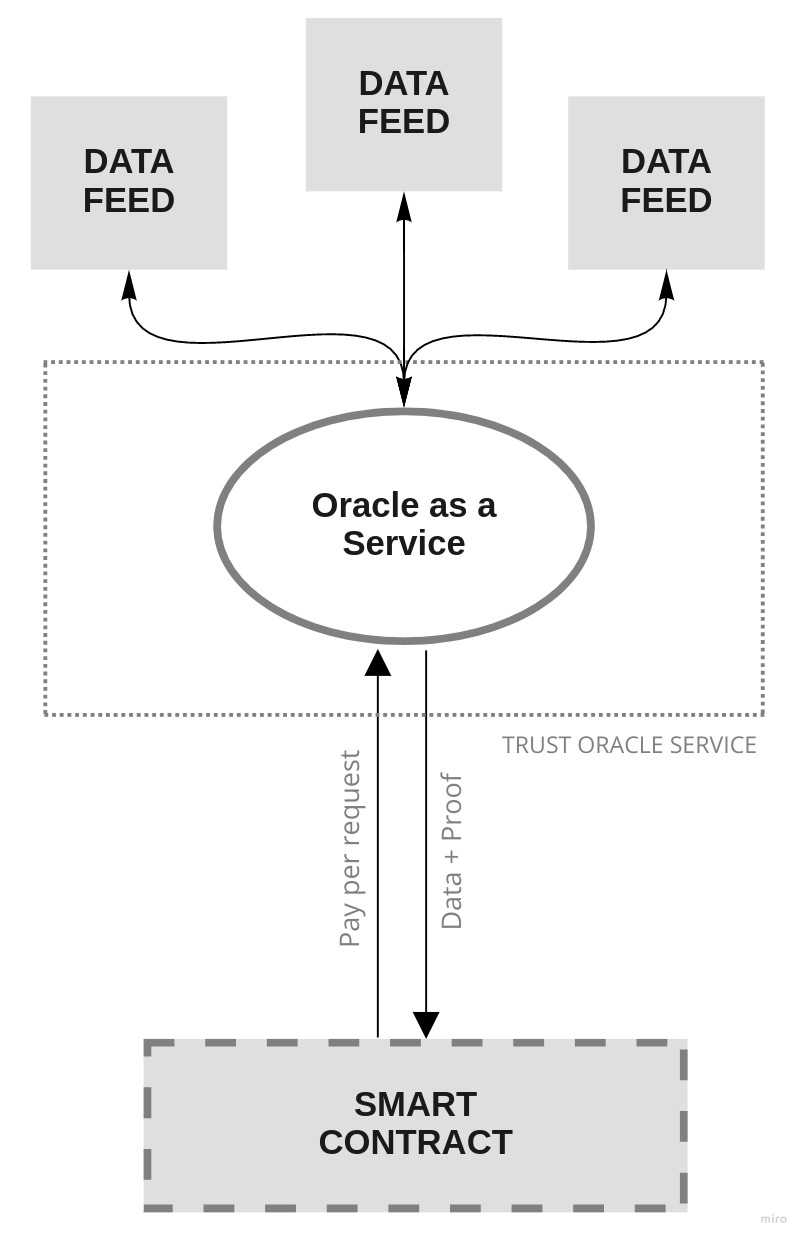
\includegraphics[width=0.5\textwidth]{figures/oraclearch2.jpg}
    \caption{Oracle as a Service w/ Multiple Data Feeds.}
    \label{fig:/figures/OaaSwMultipleDataFeed}
  \end{center}
\end{figure*}

\subsection{Example Resolved}

\subsection{Resulting Context}
In this context, the layer of trust regarding the data-feed is almost eliminated by having the ability to choose from several data providers and therefore not relying on a source of truth. It also provides a higher system availability, as the oracle/smart contract can have some degree of redundancy in the data providers selection.

\subsection{Known Uses}

\section{Single-Party Self Hosted Oracle.}\label{SPSelfHostedOracle}

\subsection{Context}
Although the use of Oracles as a Service allows for a lower product time to market by not having to take care of the development, maintenance and deployment of the oracle service it usually leads to less flexibility in the oracle design, vendor lock-in and fees charged by the vendor. If the product requirements do not allow for the specified challenges or the trust levels required by the contract are more than what the oracle vendor can provide it may be a solution to deploy its own oracle. A company with its own developing team capable of allocating resources for the development of the oracle or a single developer who does not want to incur in the oracle vendor fees will benefit from their own deployment in terms of cost and most importantly in regard to trusting the oracle behaviour.

Instead of fast-time to market the main focus here is trusting the oracle provider to behave correctly. The smart contract output will only affect a single party or multiple parties which are non competing and therefore trust someone to run the oracle. In such scenario, costs can be reduces, with increasing developer workload, by not using any authenticity proofs and the oracle can be further customised to handle a specific contract requirement.

\subsection{Example}


\subsection{Problem}
Currently, oracle behaviour is neither easy to check nor fully transparent and trustable. As seen in Chapter \ref{chap:chap4}, verifying oracles authenticity proofs sometimes cannot be done on-chain, resulting in a contract being executed with an incorrect proof which is only later verified but the contract is irreversible adding not much to oracle trustability except the ability to cancel future contracts. Proofs also add complexity to the smart contract code which will result in slower contract development and more importantly in higher contract costs. Most blockchains charge contracts by either CPU, memory and network use, or even all of these, and therefore receiving the proof and verifying it on-chain will increase the cost of running a contract.

\subsection{Forces}
\begin{itemize}
  \item \textbf{Trust} - Higher trust requirements than those provided by the authenticity proofs.
  \item \textbf{Cost optimization} - Checking authenticity proofs leads to higher contract deployment costs, as the proof can be long and computationally expensive. The use of authenticity proofs also increases personal cost, as it requires higher knowledge of the proofs workings and of cryptography.
\end{itemize}

\subsection{Solution}
A solution to trusting an oracle service is to deploy our own oracle service. Surely, doing so incurs in technical expenses for programming, deploying and maintaining the oracle, however, does not require to trust in a third party but only on our ability to maintain the necessary level of security in our own oracle. Additionally, it will free the smart contract owner from the fees charged by the oracle provider and allow for further flexibility in adapting the oracle to new sources of information. Furthermore, it will also lead to simpler and cheaper smart contracts by not requiring the use of authenticity proofs in regards to the oracle behaviour, as the developer knows exactly what the oracle is running under the hood.

\begin{figure*}[t]
  \begin{center}
    \leavevmode
    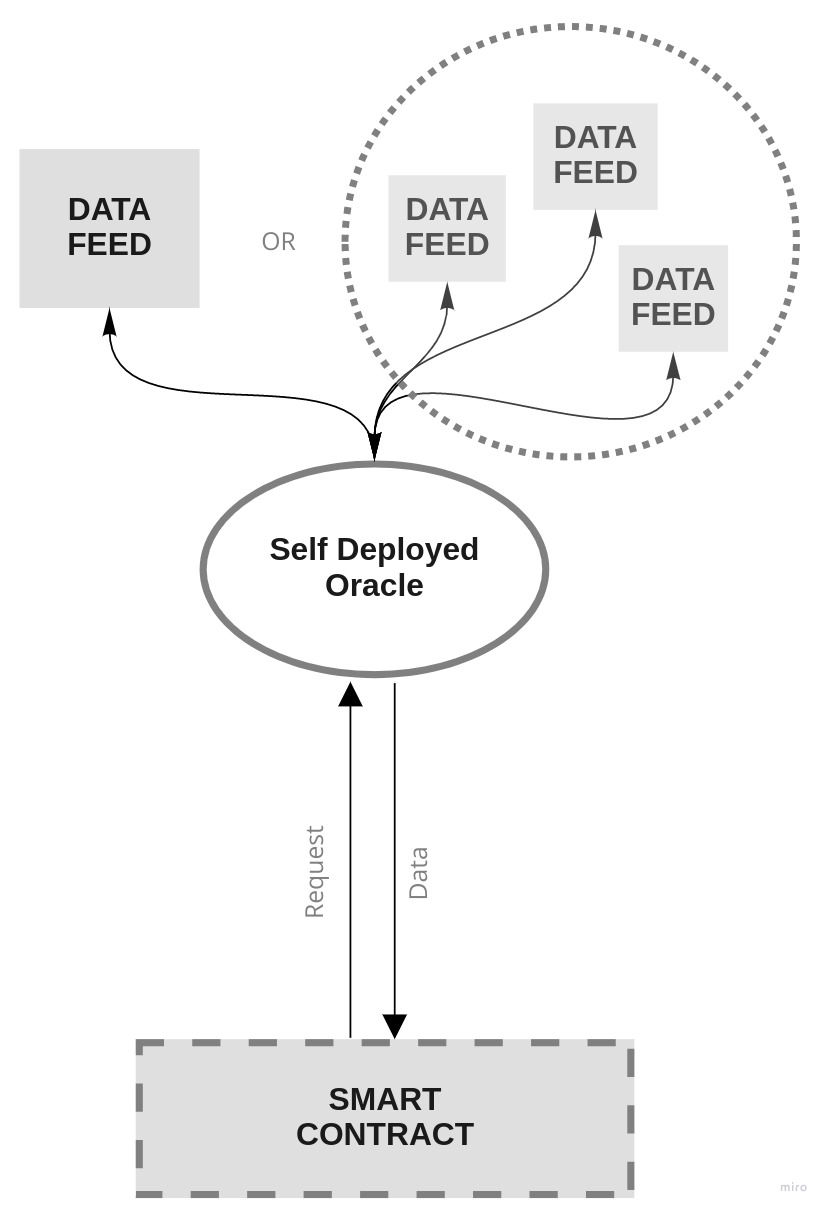
\includegraphics[width=0.5\textwidth]{figures/oraclearch3.jpg}
    \caption{Single-Party Self Hosted Oracle.}
    \label{fig:/figures/SPSelfHostedOracle}
  \end{center}
\end{figure*}


\subsection{Example Resolved}
\subsection{Resulting Context}
With this solution we almost remove the second layer of trust, trusting in the oracle service. Nonetheless, we move the trust to the developer ability in coding a secure and reliable oracle. The main benefit is not requiring to have the overhead expense of using, understanding and verifying the authenticity proofs required for a trustable use of Oracles as a service.

\subsection{Known Uses}

\section{Multi-Party Self Hosted Oracle.}\label{MPSelfHostedOracle}

\subsection{Context}
In some cases, competing parties may rely on a smart contract to keep track of some value with interest to them, therefore, it may be a requirement that several of these parties take part in the process of providing the data to the smart contract. It may also be the case, that if a single oracle is the source of truth of a smart contract, then the easiest way to attack the smart contract is by attacking the central point of failure, the oracle. In both of these cases, the oracle singularity needs to be tackled.

\subsection{Example}

\subsection{Problem}
This context raises two problems, oracle consensus and availability. Whoever owns the oracle providing the data to the smart contract holds the smart contract and therefore can influence the execution of the contract, in which several competing parties rely upon. In terms of availability, a single oracle creates a single point of failure in case of an attack or system failure.

\subsection{Forces}
\begin{itemize}
  \item \textbf{Availability} - Oracle decentralization eliminates the oracle service as a single point of failure and possible denial-of-service attacks.
  \item \textbf{Trust} - Oracle ownership decentralization brings increased trust in the result of the smart contract, as it requires multiple distinct entities to deploy an oracle and have their say in the final data provided by the oracle to the smart contract.
\end{itemize}

\subsection{Solution}
The most beneficial and simple solution, here, is having each interested party launching their own oracle and having all oracles communicating between themselves with a mechanism for consensus. The consensus mechanism would vary from case to case, and from how critical the smart contract solution is.
To increase the level of trust in each party, each node would sign their response and be able to launch only one node. With this, once one of the nodes had collected all the signatures than it would provide the contract with the requested information. Also, a party would not be able to gain control over the network of oracles by launching more nodes than the remaining stakeholders.
However, the consensus algorithm should never require that all nodes provide a response since that would again create a weak network in which by tacking down one oracle the whole system would fail.


\begin{figure*}[t]
  \begin{center}
    \leavevmode
    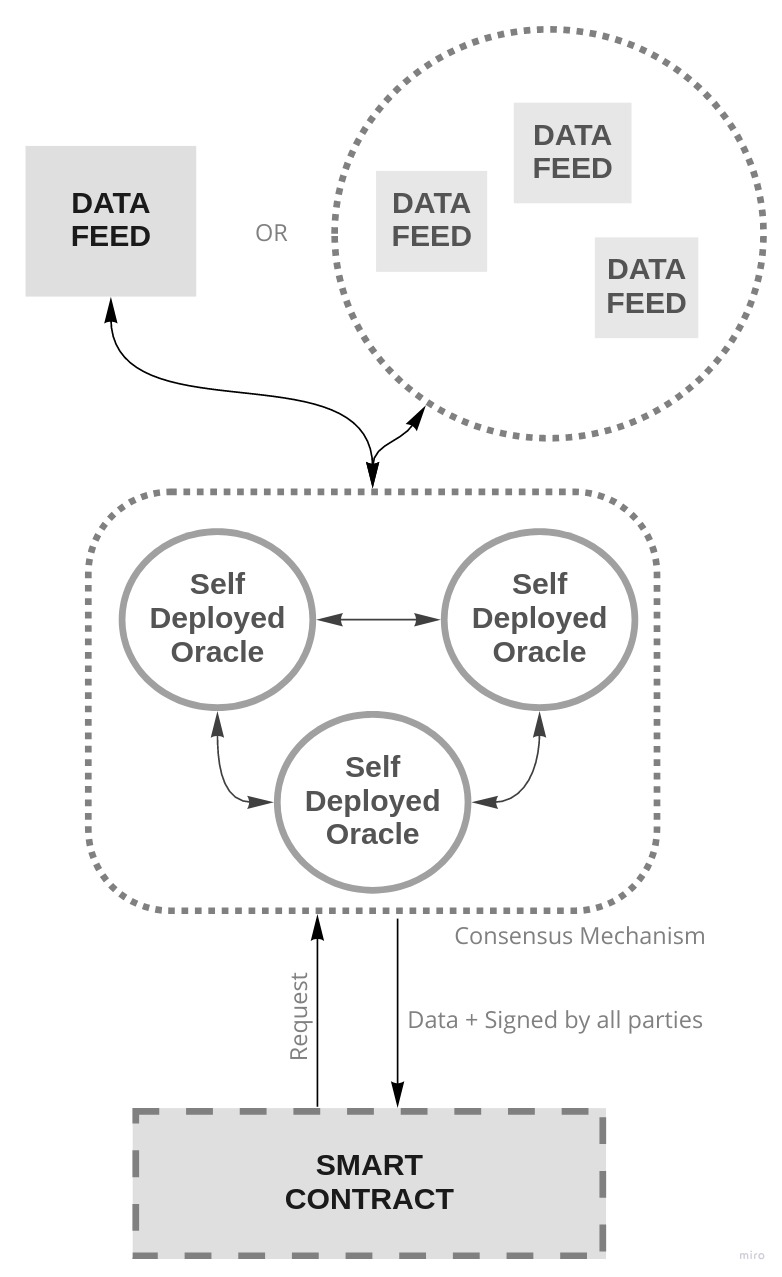
\includegraphics[width=0.5\textwidth]{figures/oraclearch4.jpg}
    \caption{Multi-Party Self Hosted Oracle.}
    \label{fig:/figures/MPSelfHostedOracle}
  \end{center}
\end{figure*}

\subsection{Example Resolved}
\subsection{Resulting Context}
With this context, we bring the same trust level given by blockchain technology to the oracle service. Resulting in a decentralized network with no single party running it and every stakeholder has the same weight in providing the data. This context, however, is only suitable for previously defined user groups, with an agreed minimum necessary quorum for consensus and known public keys of all nodes.

In a community context, this approach is not suitable since nodes would be able to join and leave making it harder to achieve a predefined consensus. Involved parties would be able to launch more than one node, resulting in some parties being able to take over the minimum consensus quorum and overpower the network unless some proof-of-work mechanism is implemented. This would also result in a context of wisdom of the crowd, in which the most effective way of controlling a correct answer would be by implementing some incentives mechanism such as \cite{Adler2018a}. The problem around incentives is that they do not guarantee that, in edge cases, with enough incentives, the network will provide a wrong answer if justifiable. Although, as far as the author is concerned, no other mechanism is available when dealing with wisdom-of-the-crowd information.



\subsection{Known Uses}


\section{Summary and Conclusions}
The described patterns represent different trust level requirements and forces. Each resolve a specific issue and may create another. When the trust requirements increase so does the gap from idea to market and development costs. Each architecture involves trading cost and flexibility with trust.

Figure \ref{fig:/figures/oracle-pattern-flow} depicts a possible simple flow of thought when choosing the previous defined pattern that better fits a specific need.

First the decision maker must look at the smart contract needs and decide if the level of trust and audibility provided by an oracle service is sufficient. If so, then can he trust the data source or is there a need for several data providers? Leaving two patterns, \ref{OaaSwSingleDataFeed} and \ref{OaaSwMultipleDataFeed}.
If he cannot trust any existing oracle service, either because the existing proofs are to expensive to verify, or cannot be verified in the contract or just don't provide the necessary audibility, among others, whatever the reason he needs to think if he has the, either monetary and human, to build his own oracle service. If not, and with increasing costs due to per-request fees, he may choose to use multiple oracle services and then perform some consensus mechanism on the smart contract. If he can then build and maintain its own oracle service he must aks him self the question, Who will use this oracle? How many different and maybe competing parties rely on the smart contract to which the oracle will provide data. If there is only one stakeholder of the smart contract and he runs the oracle, then a perfect system of trust is achieved since outside the blockchain he controls every part of the process, resulting in the pattern \ref{SPSelfHostedOracle}. However if a smart contract has several stakeholders then, no single party should control the oracle and there must be a mechanism to deploy several oracles to power the smart contract while achieving consensus outside of the blockchain and only providing the smart contract with the final result. This reduces smart contract costs while allowing every stakeholder to have a say in the data provided to the smart contract, pattern \ref{MPSelfHostedOracle}.

\begin{figure*}[t]
  \begin{center}
    \leavevmode
    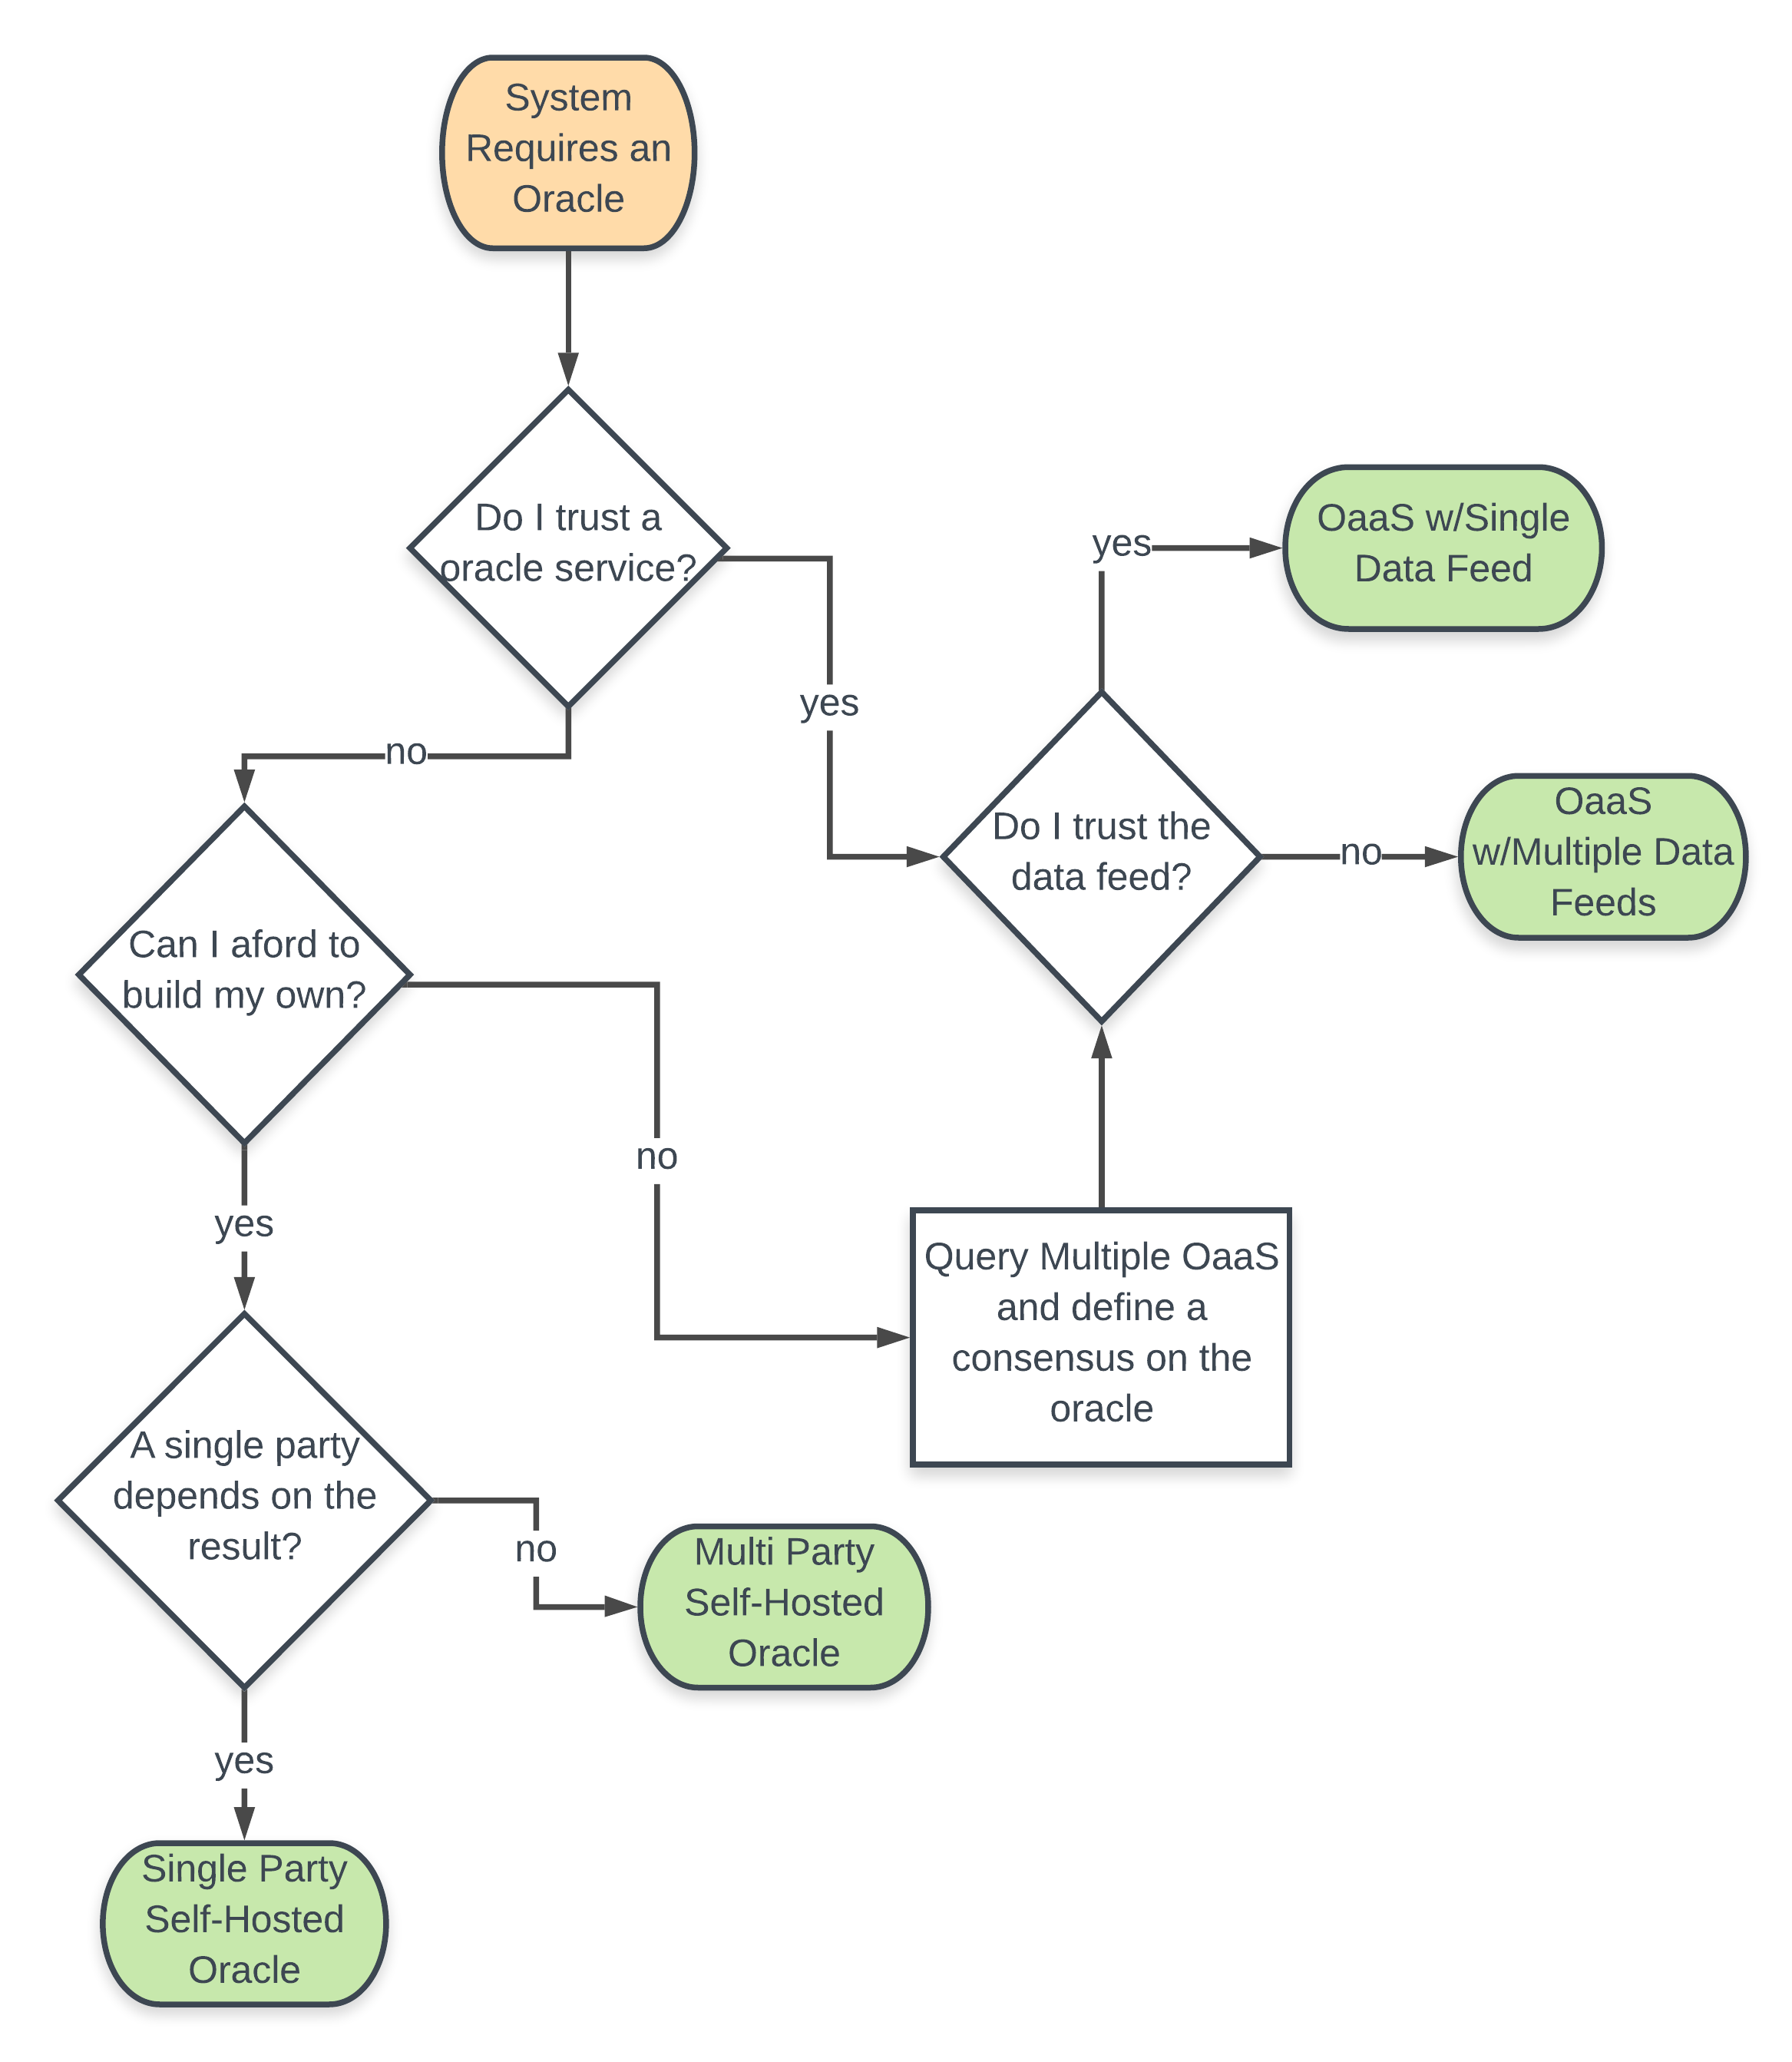
\includegraphics[width=0.8\textwidth]{figures/oracle-pattern-flow.png}
    \caption{Process for choosing the architecture of a blockchain oracle.}
    \label{fig:/figures/oracle-pattern-flow}
  \end{center}
\end{figure*}


%% Add two diagrams:
%% - flow of architecture choice -  done
%% - quadrandt inputing each architecture on a two axys: trust and complexity
 

%%----------------------------------------
%% Final materials
%%----------------------------------------

%% Bibliography
%% Comment the next command if BibTeX file not used
%% bibliography is in ``myrefs.bib''
\PrintBib{myrefs}

%% comment next 2 commands if numbered appendices are not used
\appendix
\chapter{SLR Screening Stages} \label{ap1:slr}

% Please add the following required packages to your document preamble:
% \usepackage{booktabs}
% \usepackage[normalem]{ulem}
% \useunder{\uline}{\ul}{}
% \usepackage{lscape}
% \usepackage{longtable}
% Note: It may be necessary to compile the document several times to get a multi-page table to line up properly
\begin{landscape}
    \begin{longtable}{
        @{}
        p{1cm}
        p{1cm}
        p{1cm}
        p{1.7cm}
        p{1.5cm}
        p{1cm}
        p{8cm}
        p{6.5cm}
        @{}
        }
    \toprule
    3rd screen & 2nd screen & 1st Screen & Remove Duplicates & Source & Year & Title & Authors \\* \midrule
    \endfirsthead
    %
    \multicolumn{8}{c}%
    {{\bfseries Table \thetable\ continued from previous page}} \\
    \toprule
    3rd screen & 2nd screen & 1st Screen & Remove Duplicates & Source & Year & Title & Authors \\* \midrule
    \endhead
    %
    \bottomrule
    \endfoot
    %
    \endlastfoot
    %
     &  &  & Duplicate & ACM & 2016 & Weaver: A High-performance, Transactional Graph Database Based on Refinable Timestamps & Ayush Dubey and Greg D. Hill and Robert Escriva and Emin G\&\#252;n Sirer \\
     &  &  & Duplicate & ACM & 2016 & Town Crier: An Authenticated Data Feed for Smart Contracts & Fan Zhang and Ethan Cecchetti and Kyle Croman and Ari Juels and Elaine Shi \\
     &  &  & Duplicate & ACM & 2016 & Proof of Luck: An Efficient Blockchain Consensus Protocol & Mitar Milutinovic and Warren He and Howard Wu and Maxinder Kanwal \\
     &  &  & Duplicate & ACM & 2017 & PlaTIBART: A Platform for Transactive IoT Blockchain Applications with Repeatable Testing & Michael A. Walker and Abhishek Dubey and Aron Laszka and Douglas C. Schmidt \\
     &  &  & Duplicate & ACM & 2018 & Ouroboros Genesis: Composable Proof-of-Stake Blockchains with Dynamic Availability & Christian Badertscher and Peter Ga\&\#382;i and Aggelos Kiayias and Alexander Russell and Vassilis Zikas \\
     &  &  & Duplicate & ACM & 2017 & On the Design of Communication and Transaction Anonymity in Blockchain-based Transactive Microgrids & Jonatan Bergquist and Aron Laszka and Monika Sturm and Abhishek Dubey \\
     &  &  & Duplicate & ACM & 2017 & FruitChains: A Fair Blockchain & Rafael Pass and Elaine Shi \\
     &  &  & Duplicate & ACM & 2018 & ContractFuzzer: Fuzzing Smart Contracts for Vulnerability Detection & Bo Jiang and Ye Liu and W. K. Chan \\
     &  &  & Duplicate & ACM & 2016 & Bringing Secure Bitcoin Transactions to Your Smartphone & Davide Frey and Marc X. Makkes and Pierre-Louis Roman and Fran\&\#231;ois Ta\&\#239;ani and Spyros Voulgaris \\
     &  &  & Duplicate & ACM & 2017 & Blackchain: Scalability for Resource-constrained Accountable Vehicle-to-x Communication & Rens W. van der Heijden and Felix Engelmann and David M\&\#246;dinger and Franziska Sch\&\#246;nig and Frank Kargl \\
     &  &  & Duplicate & ACM & 2017 & A General Framework for Blockchain Analytics & Massimo Bartoletti and Stefano Lande and Livio Pompianu and Andrea Bracciali \\
     &  &  & Duplicate & ACM & 2017 & EPBC: Efficient Public Blockchain Client for Lightweight Users & Lei Xu and Lin Chen and Zhimin Gao and Shouhuai Xu and Weidong Shi \\
     &  &  & Duplicate & ACM & 2016 & Blockchains and the Logic of Accountability: Keynote Address & Maurice Herlihy and Mark Moir \\
     &  &  & Duplicate & ACM & 2017 & A Byzantine Fault-tolerant Ordering Service for the Hyperledger Fabric Blockchain Platform & Alysson Bessani and Jo\&\#227;o Sousa and Marko Vukoli\&\#263; \\
     &  &  & Duplicate & IEEE & 2018 & Zero-Trust Hierarchical Management in IoT & M. Samaniego; R. Deters \\
     &  &  & Duplicate & IEEE & 2018 & Secure Pub-Sub: Blockchain-Based Fair Payment With Reputation for Reliable Cyber Physical Systems & Y. Zhao; Y. Li; Q. Mu; B. Yang; Y. Yu \\
     &  &  & Duplicate & IEEE & 2018 & Secure Attribute-Based Signature Scheme With Multiple Authorities for Blockchain in Electronic Health Records Systems & R. Guo; H. Shi; Q. Zhao; D. Zheng \\
     &  &  & Duplicate & IEEE & 2018 & Privacy Improvement Architecture for IoT & E. Kak; R. Orji; J. Pry; K. Sofranko; R. Lomotey; R. Deters \\
     &  &  & Duplicate & IEEE & 2018 & Distributed Solar Self-Consumption and Blockchain Solar Energy Exchanges on the Public Grid Within an Energy Community & C. Plaza; J. Gil; F. de Chezelles; K. A. Strang \\
     &  &  & Duplicate & IEEE & 2018 & Confidential Business Process Execution on Blockchain & B. Carminati; C. Rondanini; E. Ferrari \\
     &  &  & Duplicate & IEEE & 2018 & ChainFS: Blockchain-Secured Cloud Storage & Y. Tang; Q. Zou; J. Chen; K. Li; C. A. Kamhoua; K. Kwiat; L. Njilla \\
     &  &  & Duplicate & IEEE & 2018 & Blockchain-Based IoT-Cloud Authorization and Delegation & N. Tapas; G. Merlino; F. Longo \\
     &  &  & Duplicate & IEEE & 2017 & Blockchain world - Do you need a blockchain? This chart will tell you if the technology can solve your problem & M. E. Peck \\
     &  &  & Duplicate & IEEE & 2018 & Blockchain as a Platform for Secure Inter-Organizational Business Processes & B. Carminati; E. Ferrari; C. Rondanini \\
     &  &  & Duplicate & IEEE & 2018 & Analysis of Security in Blockchain: Case Study in 51\%-Attack Detecting & C. Ye; G. Li; H. Cai; Y. Gu; A. Fukuda \\
     &  &  & Duplicate & IEEE & 2018 & An ID-Based Linearly Homomorphic Signature Scheme and Its Application in Blockchain & Q. Lin; H. Yan; Z. Huang; W. Chen; J. Shen; Y. Tang \\
     &  &  & Duplicate & IEEE & 2019 & A New Lattice-Based Signature Scheme in Post-Quantum Blockchain Network & C. Li; X. Chen; Y. Chen; Y. Hou; J. Li \\
     &  &  & Duplicate & Scopus & 2017 & Towards an economic analysis of routing in payment channel networks & Engelmann, F., Kopp, H., Kargl, F., Glaser, F., Weinhardt, C. \\
     &  &  & Duplicate & Scopus & 2018 & 13th EAI International Conference on Security and Privacy in Communication Networks, SecureComm 2017 & {[}No author name available{]} \\
     &  &  & Duplicate & Scopus & 2017 & VIBES: Fast blockchain simulations for large-scale peer-to-peer networks & Stoykov, L., Zhang, K., Jacobsen, H.-A. \\
     &  &  & Duplicate & Scopus & 2017 & HyperPubSub: a decentralized, permissioned, publish/subscribe service using blockchains & Zupan, N., Zhang, K., Jacobsen, H.-A. \\
     &  &  & Duplicate & Scopus & 2018 & Blockchain as a platform for secure inter-organizational business processes & Carminati, B., Ferrari, E., Rondanini, C. \\
     &  & - &  & ACM & 2017 & Towards an Economic Analysis of Routing in Payment Channel Networks & Felix Engelmann and Henning Kopp and Frank Kargl and Florian Glaser and Christof Weinhardt \\
     &  & - &  & ACM & 2017 & VIBES: Fast Blockchain Simulations for Large-scale Peer-to-peer Networks: Demo & Lyubomir Stoykov and Kaiwen Zhang and Hans-Arno Jacobsen \\
     &  & - &  & ACM & 2018 & StreamChain: Do Blockchains Need Blocks? & Zsolt Istv\&\#225;n and Alessandro Sorniotti and Marko Vukoli\&\#263; \\
     &  & - &  & ACM & 2018 & Sol2Js: Translating Solidity Contracts into Javascript for Hyperledger Fabric & Muhammad Ahmad Zafar and Falak Sher and Muhammad Umar Janjua and Salman Baset \\
     &  & - &  & ACM & 2018 & Scaling Byzantine Consensus: A Broad Analysis & Christian Berger and Hans P. Reiser \\
     &  & - &  & ACM & 2018 & Resource Fairness and Prioritization of Transactions in Permissioned Blockchain Systems (Industry Track) & Seep Goel and Abhishek Singh and Rachit Garg and Mudit Verma and Praveen Jayachandran \\
     &  & - &  & ACM & 2018 & Powering Software Sustainability with Blockchain & Omar Badreddin \\
     &  & - &  & ACM & 2017 & Hyperpubsub: A Decentralized, Permissioned, Publish/Subscribe Service Using Blockchains: Demo & Nejc Zupan and Kaiwen Zhang and Hans-Arno Jacobsen \\
     &  & - &  & ACM & 2017 & How Blockchains Can Help Legal Metrology & Wilson S. Melo,Jr and Alysson Bessani and Luiz F. R. C. Carmo \\
     &  & - &  & ACM & 2018 & eVIBES: Configurable and Interactive Ethereum Blockchain Simulation Framework & Aditya Deshpande and Pezhman Nasirifard and Hans-Arno Jacobsen \\
     &  & - &  & ACM & 2018 & EVA: Fair and Auditable Electric Vehicle Charging Service Using Blockchain & Jelena Pajic and Jos\&\#233; Rivera and Kaiwen Zhang and Hans-Arno Jacobsen \\
     &  & - &  & ACM & 2018 & Deconstructing Blockchains: Concepts, Systems, and Insights & Kaiwen Zhang and Roman Vitenberg and Hans-Arno Jacobsen \\
     &  & - &  & ACM & 2018 & CIDDS: A Configurable and Distributed DAG-based Distributed Ledger Simulation Framework & Mohamed Riswan Abdul Lathif and Pezhman Nasirifard and Hans-Arno Jacobsen \\
     &  & - &  & ACM & 2018 & Blockchains for Business Process Management - Challenges and Opportunities &  \\
     &  & - &  & ACM & 2018 & Blockchain Landscape and AI Renaissance: The Bright Path Forward & Hans-Arno Jacobsen and Mohammad Sadoghi and Mohammad Hossein Tabatabaei and Roman Vitenberg and Kaiwen Zhang \\
     &  & - &  & ACM & 2018 & A Federated Low-Power WAN for the Internet of Things & Mehdi Bezahaf and Ga\&\#235;tan Cathelain and Tony Ducrocq \\
     &  & - &  & ACM & 2018 & Authenticated Modular Maps in Haskell & Victor Cacciari Miraldo and Harold Carr and Alex Kogan and Mark Moir and Maurice Herlihy \\
     &  & - &  & ACM & 2018 & Attack and Vulnerability Simulation Framework for Bitcoin-like Blockchain Technologies & Fabian Sch\&\#252;ssler and Pezhman Nasirifard and Hans-Arno Jacobsen \\
     &  & - &  & Google Shoolar & 2017 & Blockchain Oracles–Einsatz der Blockchain-Technologie für Offline-Anwendungen & A Hoppe \\
     &  & - &  & Google Shoolar & 2018 & Blockchain Coupled Oracle Fusion & D Satpathy \\
     &  & - &  & Google Shoolar & 2018 & Blockchain and Consensus from Proofs of Work without Random Oracles & JA Garay, A Kiayias, G Panagiotakos \\
     &  & - &  & Google Shoolar & 2018 & Blockchain across Oracle: Understand the details and implications of the Blockchain for Oracle developers and customers & R van Mölken \\
     &  & - &  & IEEE & 2018 & Understanding Blockchain Technology: The Costs and Benefits of Decentralization &  \\
     &  & - &  & IEEE & 2018 & Towards Application Portability on Blockchains & K. Shudo; R. Kanda; K. Saito \\
     &  & - &  & IEEE & 2017 & Secure one-time biometrie tokens for non-repudiable multi-party transactions & K. Nandakumar; N. Ratha; S. Pankanti; S. Darnell \\
     &  & - &  & IEEE & 2017 & Multiclouds in an Enterprise – a Love-Hate Relationship & M. Yousif \\
     &  & - &  & IEEE & 2019 & Leveraging the Capabilities of Industry 4.0 for Improving Energy Efficiency in Smart Factories & N. Mohamed; J. Al-Jaroodi; S. Lazarova-Molnar \\
     &  & - &  & IEEE & 2017 & Fostering consumers' energy market through smart contracts & I. Kounelis; G. Steri; R. Giuliani; D. Geneiatakis; R. Neisse; I. Nai-Fovino \\
     &  & - &  & IEEE & 2018 & ChainMOB: Mobility Analytics on Blockchain & B. Nasrulin; M. Muzammal; Q. Qu \\
     &  & - &  & IEEE & 2016 & Blockchains and the logic of accountability & M. Herlihy; M. Moir \\
     &  & - &  & IEEE & 2018 & Blockchain Based Security Framework for IoT Implementations & K. N. Krishnan; R. Jenu; T. Joseph; M. L. Silpa \\
     &  & - &  & IEEE & 2018 & Blockchain Based Vehicular Data Management & R. Sharma; S. Chakraborty \\
     &  & - &  & Scopus & 2016 & Weaver: A high-performance, transactional graph database based on refinable timestamps & Dubey, A., Hill, G.D., Sirer, E.G., Escriva, R. \\
     &  & - &  & Scopus & 2018 & Towards a smart contract-based, decentralized, public-key infrastructure & Patsonakis, C., Samari, K., Roussopoulos, M., Kiayias, A. \\
     &  & - &  & Scopus & 2016 & SysTEX 2016 - 1st Workshop on System Software for Trusted Execution, colocated with ACM/IFIP/USENIX Middleware 2016 & {[}No author name available{]} \\
     &  & - &  & Scopus & 2018 & Systematic performance evaluation using component-in-the-loop approach & Kocsis, I., Klenik, A., Pataricza, A., Telek, M., Deé, F., Cseh, D. \\
     &  & - &  & Scopus & 2018 & Synchronized aggregate signatures from the RSA assumption & Hohenberger, S., Waters, B. \\
     &  & - &  & Scopus & 2018 & Simple proofs of sequential work & Cohen, B., Pietrzak, K. \\
     &  & - &  & Scopus & 2017 & SERIAL 2017 - 1st Workshop on Scalable and Resilient Infrastructures for Distributed Ledgers, Colocated with ACM/IFIP/USENIX Middleware 2017 Conference & {[}No author name available{]} \\
     &  & - &  & Scopus & 2018 & Security of the blockchain against long delay attack & Wei, P., Yuan, Q., Zheng, Y. \\
     &  & - &  & Scopus & 2018 & Secure Pub-Sub: Blockchain-Based Fair Payment with Reputation for Reliable Cyber Physical Systems & Zhao, Y., Li, Y., Mu, Q., Yang, B., Yu, Y. \\
     &  & - &  & Scopus & 2018 & Secure Attribute-Based Signature Scheme with Multiple Authorities for Blockchain in Electronic Health Records Systems & Guo, R., Shi, H., Zhao, Q., Zheng, D. \\
     &  & - &  & Scopus & 2017 & RingCT 2.0: A compact accumulator-based (linkable ring signature) protocol for blockchain cryptocurrency Monero & Sun, S.-F., Au, M.H., Liu, J.K., Yuen, T.H. \\
     &  & - &  & Scopus & 2016 & Proof of Luck: An efficient blockchain consensus protocol & Milutinovic, M., He, W., Wu, H., Kanwal, M. \\
     &  & - &  & Scopus & 2018 & Privacy improvement architecture for IoT & Kak, E., Orji, R., Pry, J., Sofranko, K., Lomotey, R.K., Deters, R. \\
     &  & - &  & Scopus & 2017 & PlaTIBART: A Platform for Transactive IoT blockchain applications with repeatable testing & Walker, M.A., Dubey, A., Laszka, A., Schmidt, D.C. \\
     &  & - &  & Scopus & 2017 & Overcoming Cryptographic Impossibility Results Using Blockchains & Goyal, R., Goyal, V. \\
     &  & - &  & Scopus & 2018 & Ouroboros praos: An adaptively-secure, semi-synchronous proof-of-stake blockchain & David, B., Gaži, P., Kiayias, A., Russell, A. \\
     &  & - &  & Scopus & 2017 & On the design of communication and transaction anonymity in blockchain-based transactive microgrids & Bergquist, J., Laszka, A., Sturm, M., Dubey, A. \\
     &  & - &  & Scopus & 2017 & Middleware 2017 - Proceedings of the 2017 Middleware Posters and Demos 2017: Proceedings of the Posters and Demos Session of the 18th International Middleware Conference & {[}No author name available{]} \\
     &  & - &  & Scopus & 2017 & M4IoT 2017 - Proceedings of the 2017 Workshop on Middleware and Applications for the Internet of Things 4th Edition and 2nd Federated Event with the MoTA Workshop, Part of Middleware 2017 Conference & {[}No author name available{]} \\
     &  & - &  & Scopus & 2018 & IoTBDS 2018 - Proceedings of the 3rd International Conference on Internet of Things, Big Data and Security & {[}No author name available{]} \\
     &  & - &  & Scopus & 2018 & Introducing the new paradigm of Social Dispersed Computing: Applications, Technologies and Challenges & García-Valls, M., Dubey, A., Botti, V. \\
     &  & - &  & Scopus & 2017 & FruitChains: A fair blockchain & Pass, R., Shi, E. \\
     &  & - &  & Scopus & 2017 & EPBC: Efficient Public Blockchain Client for Lightweight Users & Xu, L., Chen, L., Gao, Z., Xu, S., Shi, W. \\
     &  & - &  & Scopus & 2018 & Distributed Solar Self-Consumption and Blockchain Solar Energy Exchanges on the Public Grid Within an Energy Community & Plaza, C., Gil, J., De Chezelles, F., Strang, K.A. \\
     &  & - &  & Scopus & 2018 & Designing blockchain-based SIEM 3.0 system & Miloslavskaya, N. \\
     &  & - &  & Scopus & 2018 & ChainFS: Blockchain-Secured Cloud Storage & Tang, Y., Zou, Q., Chen, J., Li, K., Kamhoua, C.A., Kwiat, K., Njilla, L. \\
     &  & - &  & Scopus & 2016 & Bringing secure Bitcoin transactions to your smartphone & Frey, D., Makkes, M.X., Roman, P.-L., Taïani, F., Voulgaris, S. \\
     &  & - &  & Scopus & 2015 & Blockchain-based model for social transactions processing & Sarr, I., Naacke, H., Gueye, I. \\
     &  & - &  & Scopus & 2018 & Blockchain-Based IoT-cloud authorization and delegation & Tapas, N., Merlino, G., Longo, F. \\
     &  & - &  & Scopus & 2017 & Blockchain world - Do you need a blockchain? This chart will tell you if the technology can solve your problem & Peck, M.E. \\
     &  & - &  & Scopus & 2017 & Blackchain: Scalability for resource-constrained accountable vehicle-to-x communication & Van Der Heijden, R.W., Engelmann, F., Mödinger, D., Schönig, F., Kargl, F. \\
     &  & - &  & Scopus & 2017 & Beyond hellman’s time-memory trade-offs with applications to proofs of space & Abusalah, H., Alwen, J., Cohen, B., Khilko, D., Pietrzak, K., Reyzin, L. \\
     &  & - &  & Scopus & 2017 & Analysis of the blockchain protocol in asynchronous networks & Pass, R., Seeman, L., Shelat, A. \\
     &  & - &  & Scopus & 2018 & Analysis of security in blockchain: Case study in 51\%-attack detecting & Ye, C., Li, G., Cai, H., Gu, Y., Fukuda, A. \\
     &  & - &  & Scopus & 2018 & An integrated platform for the Internet of Things based on an open source ecosystem & Li, Y.Q. \\
     &  & - &  & Scopus & 2018 & An ID-Based Linearly Homomorphic Signature Scheme and Its Application in Blockchain & Lin, Q., Yan, H., Huang, Z., Chen, W., Shen, J., Tang, Y. \\
     &  & - &  & Scopus & 2019 & A New Lattice-Based Signature Scheme in Post-Quantum Blockchain Network & Li, C.-Y., Chen, X.-B., Chen, Y.-L., Hou, Y.-Y., Li, J. \\
     &  & - &  & Scopus & 2017 & A general framework for blockchain analytics & Bartoletti, M., Lande, S., Pompianu, L., Bracciali, A. \\
     &  & - &  & Scopus & 2018 & A critical look at cryptogovernance of the real world: Challenges for spatial representation and uncertainty on the blockchain & Adams, B., Tomko, M. \\
     &  & - &  & Scopus & 2017 & A byzantine fault-tolerant ordering service for the hyperledger fabric blockchain platform (Short Paper) & Bessani, A., Sousa, J., Vukolić, M. \\
     &  & - &  & Scopus & 2017 & 4th International Conference on Future Data and Security Engineering, FDSE 2017 & {[}No author name available{]} \\
     &  & - &  & Scopus & 2018 & 3rd International Conference on Internet of Things, ICIOT 2018 Held as Part of the Services Conference Federation, SCF 2018 & {[}No author name available{]} \\
     &  & - &  & Scopus & 2017 & 36th Annual International Conference on the Theory and Applications of Cryptographic Techniques, EUROCRYPT 2017 & {[}No author name available{]} \\
     &  & - &  & Scopus & 2018 & 21 - Bringing down the complexity: Fast composable protocols for card games without secret state & David, B., Dowsley, R., Larangeira, M. \\
     &  & - &  & Scopus & 2018 & 13th EAI International Conference on Security and Privacy in Communication Networks, SecureComm 2017 & {[}No author name available{]} \\
     &  & - &  & Scopus & 2017 & 11th International Conference on Provable Security, ProvSec 2017 & {[}No author name available{]} \\
     & - & pass &  & ACM & 2018 & Towards Solving the Data Availability Problem for Sharded Ethereum & Daniel Sel and Kaiwen Zhang and Hans-Arno Jacobsen \\
     & - & pass &  & Google Shoolar & 2018 & Trusted agent blockchain oracle & MD Jackson \\
     & - & pass &  & IEEE & 2018 & Towards Distributed SLA Management with Smart Contracts and Blockchain & R. B. Uriarte; R. de Nicola; K. Kritikos \\
     & - & pass &  & Scopus & 2018 & Zero-trust hierarchical management in IoT & Samaniego, M., Deters, R. \\
     & - & pass &  & Scopus & 2018 & The interface between blockchain and the real world & Damjan, M. \\
     & - & pass &  & Scopus & 2018 & Ouroboros genesis: Composable proof-of-stake blockchains with dynamic availability & Badertscher, C., Gaži, P., Kiayias, A., Russell, A., Zikas, V. \\
     & - & pass &  & Scopus & 2018 & ContractFuzzer: Fuzzing smart contracts for vulnerability detection & Jiang, B., Liu, Y., Chan, W.K. \\
    - & pass & pass &  & Scopus & 2018 & Confidential Business Process Execution on Blockchain & Carminati, B., Rondanini, C., Ferrari, E. \\
    pass & pass & pass &  & ACM & 2018 & Off-chaining Models and Approaches to Off-chain Computations & Jacob Eberhardt and Jonathan Heiss \\
    pass & pass & pass &  & Google Shoolar & 2018 & Astraea: A decentralized blockchain oracle & J Adler, R Berryhill, A Veneris, Z Poulos, N Veira… \\
    pass & pass & pass &  & Google Shoolar & 2017 & Provenance and authentication of oracle sensor data with block chain lightweight wireless network authentication scheme for constrained oracle sensors & G Gordon \\
    pass & pass & pass &  & Google Shoolar & 2018 & Bitcoin gambling using distributed oracles in the blockchain & FJA Montoto Monroy \\
    pass & pass & pass &  & Scopus & 2016 & Town crier: An authenticated data feed for smart contracts & Zhang, F., Cecchetti, E., Croman, K., Juels, A., Shi, E. \\* \bottomrule
    \end{longtable}
    \end{landscape}

%% Index
%% Uncomment next command if index is required
%% don't forget to run ``makeindex mieic-en'' command
%\PrintIndex

\end{document}
